\raggedbottom
\providecolor{revisionblue}{RGB}{25,55,135}

\clearpage
\phantomsection
{\Large\bfseries Appendix Contents\par}
\vspace{1.65em}
\begingroup
\normalsize
\hypersetup{linkcolor=black}
\setlength{\parindent}{0pt}
\newcommand{\apptocsection}[3]{%
  \vspace{0.72em}\noindent
  {\large\bfseries
    \hyperref[#3]{#1\hspace{1.15em}#2}\nobreak\dotfill
    \pageref*{#3}\par}}
\newcommand{\apptocsubsection}[3]{%
  \vspace{0.28em}\noindent\hspace{2.65em}%
  \hyperref[#3]{#1\hspace{1.25em}#2}\nobreak\dotfill
  \pageref*{#3}\par}
\apptocsection{A}{Theoretical Analysis}{app:theory}
\apptocsubsection{A.1}{Proof of Theorem 1}{app:theorem-proof}
\apptocsubsection{A.2}{Theoretical Robustness}{app:theoretical-robustness}
\apptocsection{B}{Experimental Setup and Reproducibility}{app:experimental_setup}
\apptocsubsection{B.1}{Evaluation Protocol}{app:evaluation_protocol}
\apptocsubsection{B.2}{Controlled Perturbations and Distribution Shifts}{app:data_transformations}
\apptocsubsection{B.3}{Compared Methods and Task Applicability}{app:baseline_details}
\apptocsubsection{B.4}{Context Construction}{app:context_construction}
\apptocsubsection{B.5}{Implementation Details}{app:implementation_details}
\apptocsection{C}{Backbone-Wise Strength Results}{app:backbone-strength-curves}
\apptocsubsection{C.1}{TabICL-v2}{app:tabicl-strength-results}
\apptocsubsection{C.2}{Additional Backbones}{app:additional-backbone-strength-results}
\apptocsection{D}{Ablation Studies}{app:supplemental_ablations}
\apptocsubsection{D.1}{Context Budget}{app:context-budget}
\apptocsubsection{D.2}{Aggregation Rule}{app:aggregation-rule}
\apptocsubsection{D.3}{Fixed-Bank Component Ablation}{app:fixed-bank-formula-diagnostic}
\apptocsubsection{D.4}{Gate Behavior across Evidence Bins}{app:gate-bin-analysis}
\apptocsection{E}{Additional Experiments during Discussion}{app:rebuttal-additions}
\apptocsubsection{E.1}{Ensemble Comparisons}{app:revision-ensembles}
\apptocsubsection{E.2}{Larger Context Budgets}{app:revision-large-context}
\apptocsubsection{E.3}{Calibration and Constructor Matching}{app:revision-matching}
\apptocsubsection{E.4}{Unseen Mechanisms}{app:revision-unseen}
\apptocsubsection{E.5}{Natural Shifts and Repeated Runs}{app:revision-natural}
\apptocsubsection{E.6}{Robust Backbone Fine-Tuning}{app:revision-finetuning}
\apptocsubsection{E.7}{Gate Diagnostics and Extensions}{app:revision-gate}
\endgroup
\hypersetup{linkcolor=linkblue}
\clearpage

\section{Theoretical Analysis}
\label{app:theory}

\subsection{Proof of Theorem~\ref{thm:effective_context_repair}}
\label{app:theorem-proof}

\paragraph{Analysis setup and notation.}
\label{app:analysis-setup}

Let $\phi_0$ be the Base configuration and
$\Phi=\{\phi_1,\ldots,\phi_R\}$ the alternative configuration set from
Section~\ref{sec:context_interface}, indexed by
$\mathcal I(\Phi)=\{1,\ldots,R\}$. For query $i$, context $r$ produces $o_i^{(r)}$, receives
the source-calibrated prior $\pi_r$, and has bank-dependent label-free score
$\rho_i^{(r)}(\Phi)$, abbreviated below as $\rho_i^{(r)}$.
Equation~\eqref{eq:task_aware_aggregation} forms
weights $w_i^{(r)}$ and the aggregate $\bar o_i$.  The final prediction is
the task-gated mixture
\[
o_i^{\mathrm{final}}=(1-\alpha_i)o_i^{(0)}+\alpha_i\bar o_i,
\qquad
\alpha_i=\alpha_{\max}U_iE_i,
\]
where $U_i,E_i,\alpha_{\max}\in[0,1]$.

For a loss convex in its prediction argument, the context-wise and aggregate
improvements are
\[
\Delta_i^{(r)}
=\ell(o_i^{(0)},y_i^t)-\ell(o_i^{(r)},y_i^t),
\qquad
\Delta_i
=\ell(o_i^{(0)},y_i^t)-\ell(\bar o_i,y_i^t).
\]
Target labels appear only in these analysis quantities.  The construction,
weighting, and Base integration remain label-free at target inference.  We
write $P_t^{(h)}$ for the target distribution associated with change family
$h$ and $P_t$ for the target distribution used in the risk analysis.

\paragraph{Context complementarity and beneficial coverage.}
\label{app:repair-coverage}

For fixed $\delta_+>0$, define
\begin{equation}
\mathcal H_r^h
=\{i:\Delta_i^{(r)}\geq\delta_+\},
\qquad
C_h(\Phi)
  =\Pr_{P_t^{(h)}}\!\left(i\in\bigcup_{r\in\mathcal I(\Phi)}\mathcal H_r^h\right).
\label{eq:potential_repair_coverage}
\end{equation}
The set $\mathcal H_r^h$ collects the queries that context $r$ can improve
under family $h$ and is fixed once its construction and branch prediction are
fixed.  The union measures which queries have at least one beneficial context.

Adding a configuration $\phi_{r'}$ changes this coverage by
\begin{equation}
  C_h(\Phi\cup\{\phi_{r'}\})-C_h(\Phi)
  =\Pr_{P_t^{(h)}}\!\left(
    i\in\mathcal H_{r'}^h\setminus
    \bigcup_{r\in\mathcal I(\Phi)}\mathcal H_r^h
  \right).
  \label{eq:coverage_gain}
\end{equation}

\begin{lemma}[Monotone and submodular context coverage]
\label{prop:coverage_submodular}
The coverage function $C_h$ is monotone and submodular. For configuration
sets $\Phi_1\subseteq\Phi_2$ and $\phi_{r'}\notin\Phi_2$,
\begin{equation}
\begin{aligned}
0
&\leq C_h(\Phi_2\cup\{\phi_{r'}\})-C_h(\Phi_2)\\
&\leq C_h(\Phi_1\cup\{\phi_{r'}\})-C_h(\Phi_1).
\end{aligned}
\label{eq:coverage_diminishing_returns}
\end{equation}
\end{lemma}

\noindent\emph{Proof.}
Let
$\mathcal U_j=\bigcup_{r\in\mathcal I(\Phi_j)}\mathcal H_r^h$.
The marginal
coverage of $r'$ is
\[
\Pr_{P_t^{(h)}}(i\in\mathcal H_{r'}^h\setminus\mathcal U_j).
\]
Since $\mathcal U_1\subseteq\mathcal U_2$, the set difference for
$\Phi_2$ is contained in that for $\Phi_1$.  Both inequalities follow.
\hfill$\square$

Equation~\eqref{eq:coverage_diminishing_returns} characterizes potential
beneficial coverage, not realized aggregate risk. Bank-dependent scores and
gating connect coverage to risk through $\mathcal G_i$ below.

\paragraph{Score separation and effective weight.}
\label{app:evidence-separation}

Fix a bank $\Phi$, query $i$, and a nonempty effective set $\mathcal G_i$. Under
Eq.~\eqref{eq:repair_conditions}, let
\[
N_{\mathcal G}
=\sum_{r\in\mathcal G_i}\pi_r e^{\rho_i^{(r)}},
\qquad
N_{\mathcal B}
=\sum_{r\in\mathcal I(\Phi)\setminus\mathcal G_i}\pi_r e^{\rho_i^{(r)}}.
\]
Writing $\Pi_i=\sum_{r\in\mathcal G_i}\pi_r$, score separation gives
\[
N_{\mathcal G}\geq\Pi_i e^{\rho_+},
\qquad
N_{\mathcal B}\leq(1-\Pi_i)e^{\rho_-}.
\]
The normalized mass on effective contexts consequently satisfies
\begin{equation}
W_i
=\frac{N_{\mathcal G}}{N_{\mathcal G}+N_{\mathcal B}}
\geq
\left[1+\frac{1-\Pi_i}{\Pi_i}
e^{-(\rho_+-\rho_-)}\right]^{-1}
=\underline W_i.
\label{eq:appendix_effective_weight}
\end{equation}
This bound exposes two routes to a larger effective weight: greater prior
mass $\Pi_i$ and a wider score gap $\rho_+-\rho_-$.  Convexity then yields
\begin{equation}
\begin{aligned}
\Delta_i
&\geq\sum_{r=1}^{R} w_i^{(r)}\Delta_i^{(r)}\\
&\geq W_i\delta_+-(1-W_i)\delta_-\\
&\geq\underline W_i\delta_+-(1-\underline W_i)\delta_-
=\gamma_i.
\end{aligned}
\label{eq:appendix_aggregate_gain}
\end{equation}
Hence the effective contexts dominate the aggregate whenever
$\underline W_i>\delta_-/(\delta_++\delta_-)$.

The scores combine source calibration with target-side confidence, agreement,
or proximity.  Their joint ordering determines whether the separation
condition holds; the analysis below also covers imperfect ordering.

\paragraph{Proof of Theorem~\ref{thm:effective_context_repair}.}

Equation~\eqref{eq:appendix_effective_weight} proves the lower bound on
$W_i$, and Eq.~\eqref{eq:appendix_aggregate_gain} proves
$\Delta_i\geq\gamma_i$.  The condition
$\underline W_i>\delta_-/(\delta_++\delta_-)$ is equivalent to
$\gamma_i>0$.

Applying convexity to the task-gated update gives
\[
\begin{aligned}
\ell(o_i^{\mathrm{final}},y_i^t)
&\leq(1-\alpha_i)\ell(o_i^{(0)},y_i^t)
+\alpha_i\ell(\bar o_i,y_i^t),\\
\ell(o_i^{\mathrm{final}},y_i^t)-\ell(o_i^{(0)},y_i^t)
&\leq-\alpha_i\Delta_i.
\end{aligned}
\]
For $i\in\mathcal A_\Phi$, the aggregate bound therefore gives
\[
\ell(o_i^{\mathrm{final}},y_i^t)-\ell(o_i^{(0)},y_i^t)
\leq-\alpha_{\max}U_iE_i\gamma_i.
\]
For $i\notin\mathcal A_\Phi$, the same convexity inequality gives
\[
\ell(o_i^{\mathrm{final}},y_i^t)-\ell(o_i^{(0)},y_i^t)
\leq\alpha_{\max}U_iE_i(-\Delta_i)_+.
\]
Taking the $P_t$ expectation and splitting it over
$\mathcal A_\Phi$ and its complement yields
Eq.~\eqref{eq:changed_risk_gain}.  The strict risk improvement follows when
$\Gamma_t(\Phi)>\varepsilon_t(\Phi)$. \hfill$\square$

\paragraph{Interpretation: family-directed construction.}
\label{app:family-construction}

Family-directed construction enters through complementary coverage and
effective score mass. A construction adds coverage when its beneficial region
contains queries outside the union of the current regions, as quantified by
Eq.~\eqref{eq:coverage_gain}.  On a covered query, a larger effective prior
mass $\Pi_i$ or score gap $\rho_+-\rho_-$ increases the lower bound on
$W_i$ when the separation condition holds, increasing the margin $\gamma_i$.

These results connect family-directed construction, complementary coverage,
score weighting, and the task-specific gate to the risk decomposition in
Theorem~\ref{thm:effective_context_repair}. Deviations from score
separation and harmful high-support consensus are analyzed in
Appendix~\ref{app:theoretical-robustness}.

\subsection{Theoretical Robustness}
\label{app:theoretical-robustness}

\paragraph{Risk under imperfect score separation.}
\label{app:imperfect-separation}

Let $\mathcal A_\Phi$ be the beneficial-update region defined in
Theorem~\ref{thm:effective_context_repair}.  Its complement contains queries
for which the required improvement, score ordering, or aggregate margin
does not hold. Define its gate-weighted mass by
\begin{equation}
M_t(\Phi)
:=\mathbb E_{P_t}\!\left[
U_iE_i\mathbf 1\{i\notin\mathcal A_\Phi\}\right].
\label{eq:misalignment_mass}
\end{equation}

\begin{proposition}[Imperfect score separation]
\label{prop:imperfect_evidence}
Suppose $(-\Delta_i)_+\leq L_\Delta<\infty$ on the target prediction domain.
This holds, for example, when each class probability satisfies
$p_k\geq\varepsilon_p>0$ and regression targets and predictions are bounded. Then
\begin{equation}
\mathcal R_t(g_{\mathrm{final}})-\mathcal R_t(g_0)
\leq
-\Gamma_t(\Phi)+\alpha_{\max}L_\Delta M_t(\Phi).
\label{eq:imperfect_evidence_risk}
\end{equation}
\end{proposition}

\noindent\emph{Proof.}
The residual term in Eq.~\eqref{eq:repair_residual_terms} satisfies
\[
\varepsilon_t(\Phi)
\leq\alpha_{\max}L_\Delta
\mathbb E_{P_t}[U_iE_i\mathbf 1\{i\notin\mathcal A_\Phi\}].
\]
Substitution into Eq.~\eqref{eq:changed_risk_gain} proves the result.
\hfill$\square$

Proposition~\ref{prop:imperfect_evidence} requires separation on the
beneficial portion of the target distribution rather than on every query.
Score-ordering errors enter through $M_t(\Phi)$ and are attenuated by the
same task-specific and context-support gates used by the algorithm.

\paragraph{Harmful high-support consensus.}
\label{app:harmful-consensus}

Correlated alternative errors can produce high agreement around an adverse
aggregate. For a threshold $e\in[0,1]$, define the harmful high-support
consensus rate
\begin{equation}
\eta_{\mathrm{fc}}(e)
:=\Pr_{P_t}(E_i>e,\ \Delta_i<0).
\label{eq:false_consensus_rate}
\end{equation}
This event isolates confident agreement that moves the aggregate away from
the target label under the analyzed loss.

\begin{proposition}[Residual-risk refinement]
\label{prop:false_consensus}
Under the bounded adverse improvement condition of
Proposition~\ref{prop:imperfect_evidence},
\begin{equation}
\varepsilon_t(\Phi)
\leq\alpha_{\max}L_\Delta
\left[e+\eta_{\mathrm{fc}}(e)\right].
\label{eq:false_consensus_bound}
\end{equation}
Consequently,
\begin{equation}
\mathcal R_t(g_{\mathrm{final}})-\mathcal R_t(g_0)
\leq-\Gamma_t(\Phi)
+\alpha_{\max}L_\Delta
\left[e+\eta_{\mathrm{fc}}(e)\right].
\label{eq:false_consensus_risk}
\end{equation}
\end{proposition}

\noindent\emph{Proof.}
Dropping the indicator of $\mathcal A_\Phi^c$ only enlarges the residual.
Split the remaining expectation at $E_i=e$.  On $E_i\leq e$,
$U_iE_i(-\Delta_i)_+\leq eL_\Delta$.  On $E_i>e$, a positive contribution
requires $\Delta_i<0$, while $U_iE_i(-\Delta_i)_+\leq L_\Delta$.
Taking expectations gives Eq.~\eqref{eq:false_consensus_bound}; combining it
with Eq.~\eqref{eq:changed_risk_gain} gives
Eq.~\eqref{eq:false_consensus_risk}. \hfill$\square$

Equation~\eqref{eq:false_consensus_bound} is a conservative decoupled bound
obtained with $U_i\leq1$; Eq.~\eqref{eq:repair_residual_terms} retains $U_i$.

The bound divides residual harm into low-support updates, controlled by
$e$, and harmful high-support consensus, controlled by
$\eta_{\mathrm{fc}}(e)$. Complementary contexts can enlarge
$\Gamma_t(\Phi)$, whereas repeated adverse agreement contributes to
$\eta_{\mathrm{fc}}(e)$.

\paragraph{Base-deviation bounds.}
\label{app:base-preservation}

The update in Eq.~\eqref{eq:base_anchored_update} satisfies the exact identity
\[
o_i^{\mathrm{final}}-o_i^{(0)}
=\alpha_{\max}U_iE_i(\bar o_i-o_i^{(0)}).
\]
Thus the final prediction recovers Base whenever $U_iE_i=0$, and otherwise
its displacement is scaled by the product of the two gates.

For classification,
\[
p_i^{\mathrm{final}}-p_i^{(0)}
=\alpha_i(\bar p_i-p_i^{(0)}).
\]
The homogeneity of total variation, together with
$\operatorname{TV}(\bar p_i,p_i^{(0)})\leq1$ and
$E_i^{\mathrm{cls}}\leq1$, yields
\begin{equation}
\operatorname{TV}(p_i^{\mathrm{final}},p_i^{(0)})
\leq\alpha_i
\leq\alpha_{\max}\frac{H(p_i^{(0)})}{\log L}.
\label{eq:classification_preservation}
\end{equation}
Let $M_i^{(0)}$ be the gap between the largest and second-largest Base class
probabilities.  Since each probability changes by at most
$\alpha_i\lVert\bar p_i-p_i^{(0)}\rVert_\infty$, the predicted class remains
unchanged whenever
\begin{equation}
2\alpha_i\lVert\bar p_i-p_i^{(0)}\rVert_\infty<M_i^{(0)}.
\label{eq:classification_margin_preservation}
\end{equation}

For regression, $U_i$ is the Base-aggregate discrepancy gate. Let
$d_i=|\bar y_i-\hat y_i^{(0)}|$. Since
$E_i^{\mathrm{reg}}\leq1$ and $1-e^{-x}\leq x$ for $x\geq0$,
\begin{equation}
\begin{aligned}
|\hat y_i^{\mathrm{final}}-\hat y_i^{(0)}|
&=\alpha_i d_i\\
&\leq\alpha_{\max}\left(1-e^{-d_i/\tau_y}\right)d_i\\
&\leq\frac{\alpha_{\max}}{\tau_y}d_i^2.
\end{aligned}
\label{eq:regression_preservation}
\end{equation}
Equations~\eqref{eq:classification_preservation}--\eqref{eq:regression_preservation}
are the task-specific forms of the Base-deviation identity in
Eq.~\eqref{eq:base_preservation_identity}.

\section{Experimental Setup and Reproducibility}
\label{app:experimental_setup}
\label{app:experimental_details}

\subsection{Evaluation Protocol}
\label{app:evaluation_protocol}

\subsubsection{Benchmarks and Evaluation Splits}
\label{app:data_splits}

We use complementary public-data and fully synthetic evaluation tracks.  The
public-data track further separates five controlled context perturbations from
seven distribution shifts.  Table~\ref{tab:public-benchmark-protocols}
summarizes the fixed task sets and sample protocols.

\begin{table}[H]
  \caption{Public-data benchmark composition and fixed sample protocols.  A
  cap is an upper bound; smaller official folds retain all available rows.}
  \label{tab:public-benchmark-protocols}
  \centering
  \footnotesize
  \setlength{\tabcolsep}{4pt}
  \begin{tabular}{@{}>{\raggedright\arraybackslash}p{0.14\textwidth}
                      >{\raggedright\arraybackslash}p{0.39\textwidth}
                      >{\raggedright\arraybackslash}p{0.39\textwidth}@{}}
    \toprule
    Track & Classification & Regression \\
    \midrule
    Controlled context perturbations
      & All 72 OpenML-CC18 tasks, including binary and multiclass tasks.  Each
        task uses 384 fixed rows: 256 labeled source-context rows and 128 target
        evaluation rows.
      & All 35 OpenML-CTR23 tasks.  The official source and target partitions
        are capped at 2,048 and 512 rows, respectively. \\
    Distribution shifts
      & A fixed 35-task binary subset of OpenML-CC18.  Each task uses 256
        historical source rows, 64 reference rows, and 128 target evaluation
        rows, with a labeled context budget of 256.
      & The 33 OpenML-CTR23 tasks that support the fixed partition: at most
        1,024 source rows and 256 target rows, with 256 current-context rows,
        128 reference rows, and the remaining source rows used as history. \\
    \bottomrule
  \end{tabular}
\end{table}

The distribution-shift regression track excludes \nolinkurl{forest_fires} and
\nolinkurl{student_performance_por}.  Their official training folds contain
fewer than 640 rows and therefore cannot support disjoint current, reference,
and historical partitions under the fixed budget.

Public-data policy selection uses five-fold \emph{dataset-level} out-of-fold
(OOF) evaluation. The outer folds partition complete datasets rather than rows.
For each held-out dataset, context configurations and the fusion policy are
determined using datasets in the other four folds and then frozen; only
preprocessing and constructor statistics are recomputed from its source context.
All methods share the same dataset folds and base source--target partition.
For each problem family, we evaluate strengths
$s\in\{0,0.2,0.5,0.8,1.0\}$; $s=0$ preserves the original context and inputs.
Within a sweep, feature maps retain target row identities, while the label-shift
operator resamples complete rows from fixed class-specific target pools.

The fully synthetic track uses five response mechanisms---linear,
interaction, smooth nonlinear, threshold, and subgroup.  Seed 0 is used for
method development, whereas the reported confirmation results use previously
unseen seeds 4, 5, and 6.  Each condition contains 512 source rows and 384
target rows with a fixed 256-row labeled context.  Within a
seed--DGP--scenario unit, all methods and strengths reuse the same base samples,
random streams, and context indices.  The five DGPs, three confirmation seeds,
and twelve non-clean problem families yield $5\times3\times12=180$ aligned
evaluation units.  Section~\ref{app:data_transformations} specifies the
generators and transformations.

\subsubsection{Metrics and Statistical Reporting}
\label{app:metrics_reporting}

Classification is evaluated with Accuracy and AUROC, and regression with
$R^2$, normalized mean absolute error (nMAE), and normalized root mean squared
error (nRMSE).  Higher is better for Accuracy, AUROC, and $R^2$; lower is
better for nMAE and nRMSE.  AUROC and $R^2$ are the primary metrics for the
robustness rankings and strength--response analyses.

For target values $y_i$ and predictions $\hat y_i$, let
\begin{equation}
  \operatorname{MAE}=\frac{1}{n}\sum_{i=1}^{n}|y_i-\hat y_i|,
  \qquad
  \operatorname{RMSE}=\sqrt{\frac{1}{n}\sum_{i=1}^{n}(y_i-\hat y_i)^2}.
\end{equation}
We report
\begin{equation}
  \operatorname{nMAE}=\frac{\operatorname{MAE}}{\max(\sigma,10^{-12})},
  \qquad
  \operatorname{nRMSE}=\frac{\operatorname{RMSE}}{\max(\sigma,10^{-12})},
\end{equation}
where the frozen benchmark implementations use
\begin{equation}
  \sigma=
  \begin{cases}
    \operatorname{std}(y_{\mathrm{source}}),
      & \text{controlled context perturbations},\\
    \operatorname{std}(y_{\mathrm{target}}),
      & \text{distribution shifts}.
  \end{cases}
\end{equation}
Both are population standard deviations (\texttt{ddof=0}).  Because the two
tracks use different normalization scales, nMAE and nRMSE are compared only
within a track; cross-track regression summaries use $R^2$.  In the shift
track, $\operatorname{std}(y_{\mathrm{target}})$ is computed only after all
predictions have been produced and is used solely for metric evaluation.

For public data, we compute one dataset-level OOF score per condition and then
macro-average across datasets, giving every dataset equal weight.  A summary
over several problem families first averages dataset-level scores within each
family and strength and then takes an equal-weight mean over the five context
perturbations or seven distribution shifts. Reported public-data curves use only
observed points, without smoothing, fitting, or monotonic projection.

Synthetic confidence intervals use 10,000 nonparametric bootstrap resamples
with replacement and the 2.5th and 97.5th percentiles of the bootstrap means.
The resampling unit is a complete seed--DGP--scenario unit rather than an
individual row.  The clean anchor contains $3\times5=15$ units; each nonzero
controlled-perturbation point contains $3\times5\times5=75$ units; each nonzero
distribution-shift point contains $3\times5\times7=105$ units; and the
twelve-family summary contains 180 units.

For the pairwise stability analysis, we average each metric over the four
nonzero strengths within a seed--DGP--scenario unit. Writing AUROC as AUC, the
normalized classification and regression degradations are
\begin{equation}
  d_{\mathrm{cls}}
  =\frac{\mathrm{AUC}_{\mathrm{clean}}-\mathrm{AUC}_{\mathrm{shift}}}
  {\max(\mathrm{AUC}_{\mathrm{clean}}-0.5,0.05)},
  \qquad
  d_{\mathrm{reg}}
  =\frac{R^2_{\mathrm{clean}}-R^2_{\mathrm{shift}}}
  {\max(|R^2_{\mathrm{clean}}|,0.1)}.
\end{equation}
For each method pair, the smaller degradation counts as a win; absolute
differences no greater than $0.001$ are counted as ties.

\subsubsection{Leakage Control}
\label{app:leakage_control}

The dataset-level OOF design separates policy selection from held-out-dataset
evaluation. For a held-out dataset, fusion weights and other data-dependent
policy parameters are determined from the other four folds and then frozen.
Constructors may use the labeled source context available to the method, and
target-aware constructors may additionally inspect unlabeled target features
$X_t$, but never target labels.

Held-out labels are not used for context construction, candidate selection,
fusion-policy fitting, or prediction.  They are accessed only after prediction
to compute the reported metrics.  Metadata visibility is fixed by the method
interface: Shared uses a family-agnostic context registry, whereas the
prior-informed Specific variant may receive the problem-family identifier
specified before target inference.  Section~\ref{app:regression_evidence}
details candidate selection and aggregation for each interface.

\subsection{Controlled Perturbations and Distribution Shifts}
\label{app:data_transformations}

\subsubsection{Common Design}

We express every intervention as a deterministic, severity-indexed operator
$\mathcal T_s$, where $s\in\{0,0.2,0.5,0.8,1.0\}$ and $\mathcal T_0$ is the
identity.  For a source-context perturbation, $s$ determines the affected-row
count $m_s=\lceil s n_c\rceil$ for $s>0$; for a distribution shift, it controls
either a nested replacement fraction or the magnitude of a feature or response
map.  Within a dataset--family pair, the clean partition and base cohort are
fixed, and every random seed is a deterministic function of the registered
condition.  No split, model, or policy is retuned along a strength curve.

The synthetic track draws $X\sim\mathcal N(0,\Sigma)$ in 12 dimensions, where
$\Sigma_{jj}=1$, $\Sigma_{12}=\Sigma_{21}=0.35$,
$\Sigma_{34}=\Sigma_{43}=-0.25$, and all other off-diagonal entries are zero.
It uses five fixed response mechanisms---linear, pairwise interaction, smooth
nonlinear, threshold, and two-subgroup piecewise linear---with the same active
coordinates and coefficients across all methods, strengths, and seeds.
For each generated block, $g(x)=h(x)-\operatorname{median}\{h(X)\}$.
Classification draws $Y\sim\operatorname{Bernoulli}(\operatorname{sigmoid}(g(X)))$;
regression uses $Y=g(X)+\epsilon$ with
$\epsilon\sim\mathcal N(0,0.65^2)$. The rotated concept rule reverses the
first five signal coordinates. The public-data track starts from the fixed OpenML partitions in
Table~\ref{tab:public-benchmark-protocols} and applies empirical resampling or
feature/response transformations.  Consequently, distributional equalities
below describe the synthetic construction; their OpenML counterparts preserve
the corresponding variables or row identities by design, rather than asserting
exact finite-sample equality.

\subsubsection{Controlled Source-Context Perturbations}

Let $j^\star$ denote the feature with the largest absolute source
feature--target association.  For each family, a deterministic rule selects a
subset $I_s$ of $m_s$ source rows; score-ranked families are nested across
severity, whereas Mixed uses a seeded subset at each severity.  Only
$(X_c,y_c)$ on these rows is modified; the target evaluation cohort and its
labels are unchanged.
Table~\ref{tab:context-perturbation-transformations} gives the complete
operator-level description.

\begin{table}[H]
  \caption{Controlled transformations of the labeled source context.  Label
  cycling applies only to classification; opposite-tail response replacement
  applies only to regression.}
  \label{tab:context-perturbation-transformations}
  \centering
  \footnotesize
  \setlength{\tabcolsep}{3pt}
  \begin{tabular}{@{}>{\raggedright\arraybackslash}p{0.12\textwidth} >{\raggedright\arraybackslash}p{0.25\textwidth} >{\raggedright\arraybackslash}p{0.56\textwidth}@{}}
    \toprule
    Family & Affected-row rule & Transformation on selected rows \\
    \midrule
    Shortcut
      & Decreasing absolute label/response deviation from its median.
      & Replace $X_{j^\star}$ by a strong value on the side opposite to the
        observed label or response; $y$ is retained. \\
    Boundary
      & Increasing distance to empirical label/response quartile cut points.
      & Classification shifts $X_{j^\star}$ against the label and cycles a
        deterministic half of the labels; regression sends responses to the
        opposite empirical tail. \\
    AUC/Rank-band
      & Increasing distance to the median of $X_{j^\star}$.
      & Classification shifts $X_{j^\star}$ and cycles every third selected
        label; regression sends selected responses to the opposite empirical
        tail. \\
    Local
      & Increasing distance to a fixed local anchor in feature space.
      & Modify both $X_{j^\star}$ and the label/response, creating a
        contradictory pattern confined to one neighborhood. \\
    Mixed
      & A seeded random subset of size $m_s$.
      & Partition the selected subset into four fixed chunks and apply
        Shortcut, Boundary, AUC/Rank-band, and Local, respectively. \\
    \bottomrule
  \end{tabular}
\end{table}

\subsubsection{Distribution-Shift Families}

For the synthetic track, let $Z$ denote latent features,
$g_{\mathrm{rot}}$ a response rule with reordered signal coordinates, and
$T_s$ a severity-controlled observation map.  Table~\ref{tab:shift-transformations}
first states the intended distributional change and then records its
classification and regression OpenML realizations.  The public classification
protocol can transform the historical/reference source blocks or the target
block, whereas the public regression protocol transforms the current labeled
context against a fixed target cohort; this distinction follows the sample
interfaces in Table~\ref{tab:public-benchmark-protocols}.

\begin{table}[H]
  \caption{Seven source--target shift families.  The invariant column describes
  the synthetic population construction; the last two columns specify the
  empirical OpenML operators.}
  \label{tab:shift-transformations}
  \centering
  \scriptsize
  \setlength{\tabcolsep}{2.5pt}
  \begin{tabular}{@{}>{\raggedright\arraybackslash}p{0.09\textwidth}
                      >{\raggedright\arraybackslash}p{0.22\textwidth}
                      >{\raggedright\arraybackslash}p{0.30\textwidth}
                      >{\raggedright\arraybackslash}p{0.30\textwidth}@{}}
    \toprule
    Family & Synthetic change / invariant & OpenML classification & OpenML regression \\
    \midrule
    Covariate
      & Change $P(X)$ while retaining $P(Y\mid X)$.
      & Resample historical/reference rows with an $X$-only weight; keep the
        target cohort fixed.
      & Replace a nested fraction of current-context rows along the
        highest-variance feature; keep the target fixed. \\
    Label
      & Change $P(Y)$ while retaining $P(X\mid Y)$.
      & Resample complete target rows within class to vary the class prior.
      & Resample complete current-context rows toward one response tail. \\
    Concept
      & Interpolate $g$ toward $g_{\mathrm{rot}}$ at fixed $P(X)$.
      & Apply nested local boundary-label changes to reference and target rows;
        features are fixed.
      & Add a smooth, feature-dependent response drift to the current context;
        features are fixed. \\
    Selection
      & Make source inclusion depend on $X$; retain $P(Y\mid X)$.
      & Resample source rows by an $X$-only predicted-majority affinity; keep
        the target fixed.
      & Resample current rows by $X$-only distance from the target center. \\
    Domain
      & Use $T_0$ and $T_s$ on shared latent rows; retain $P(Y\mid Z)$.
      & Apply an affine observation map to target features; row identities and
        labels are fixed.
      & Apply an affine observation map to current-context features; responses
        are fixed. \\
    Temporal
      & Evolve both $T_s$ and the response rule while preserving temporal order.
      & Apply joint feature and local concept drift to the reference and target
        blocks; historical rows remain earlier observations.
      & Apply joint feature and response drift to the current block while
        retaining disjoint history and reference blocks. \\
    Support
      & Translate observed support while retaining $P(Y\mid Z)$.
      & Translate target coordinates; row identities and labels are fixed.
      & Resample the current context toward a restricted central support using
        an $X$-only score. \\
    \bottomrule
  \end{tabular}
\end{table}

All intervention operators are created before method evaluation.  Target labels
used to define or score a benchmark condition are never exposed to a compared
method, a context constructor, or the aggregation policy.

\FloatBarrier

\subsection{Compared Methods and Task Applicability}
\label{app:baseline_details}

We organize the compared methods by evaluation purpose.  The OpenML study
compares standard statistical, tree-based, deep tabular, and frozen
foundation-model predictors under common data partitions.  The synthetic study
focuses on methods designed for perturbations or distribution shifts.  Because
not every robustness method supports both prediction tasks, we distinguish
shared, classification-only, and regression-only baselines.  This subsection
defines the comparison set and task applicability; protocol and selection
details are separated into the surrounding appendix subsections.

\subsubsection{OpenML Baselines}

\paragraph{Classical and tree models.}
\begin{itemize}
  \setlength{\itemsep}{1pt}
  \setlength{\parskip}{0pt}
  \item \textbf{Logistic/Ridge}---regularized linear classification and
  regression~\citep{cox1958binary,hoerl1970ridge}.
  \item \textbf{SVM/SVR}---margin-based classification and
  regression~\citep{cortes1995svm,drucker1996svr}.
  \item \textbf{kNN}---classification or regression from local neighbors in
  feature space~\citep{cover1967knn}.
  \item \textbf{Random Forest}---bagged decision-tree
  ensembles~\citep{breiman2001randomforests}.
  \item \textbf{LightGBM}---histogram-based gradient-boosted
  trees~\citep{ke2017lightgbm}.
  \item \textbf{CatBoost}---gradient-boosted trees trained with ordered
  boosting~\citep{prokhorenkova2018catboost}.
  \item \textbf{XGBoost}---regularized gradient-boosted
  trees~\citep{chen2016xgboost}.
  \item \textbf{MLP}---a feed-forward neural baseline trained on each source
  fold~\citep{rumelhart1986backprop}.
\end{itemize}

\paragraph{Deep tabular models.}
\begin{itemize}
  \setlength{\itemsep}{1pt}
  \setlength{\parskip}{0pt}
  \item \textbf{FT-Transformer}---a Transformer over tokenized tabular
  features~\citep{gorishniy2021fttransformer}.
  \item \textbf{TabM}---a parameter-efficient ensemble of MLP-like
  predictors~\citep{gorishniy2025tabm}.
  \item \textbf{TabulaRNN}---an RNN-inspired architecture for efficient
  tabular learning~\citep{thielmann2024tabularnn}.
  \item \textbf{MambaTab}---a structured state-space architecture for tabular
  prediction~\citep{ahamed2024mambatab}.
  \item \textbf{RealMLP}---an MLP with a pre-tuned configuration for tabular
  data~\citep{holzmueller2024realmlp}.
\end{itemize}

\paragraph{Frozen foundation-model backbones.}
\begin{itemize}
  \setlength{\itemsep}{1pt}
  \setlength{\parskip}{0pt}
  \item \textbf{LimiX-2M}---the official checkpoint, evaluated without
  parameter updates and displayed under its full model name in the main
  table~\citep{wang2026limix2m}.
  \item \textbf{TabICL-v2}---a scalable tabular in-context learning
  model~\citep{qu2026tabiclv2}.
  \item \textbf{TabPFN-v3}---a pretrained tabular foundation
  model~\citep{grinsztajn2026tabpfn3technicalreport}.
  \item \textbf{TabDPT v1.2}---a tabular foundation model pretrained on real
  data~\citep{ma2025tabdpt}.
\end{itemize}

\paragraph{LimiX compatibility on the complete suites.}
The LimiX-2M study excludes classification datasets with more than ten target
classes and consequently reports 62 of the 72 OpenML-CC18 tasks; applying the
same filters leaves 33 OpenML-CTR23 tasks~\citep{wang2026limix2m}.  Our main
table instead targets the complete 72-task CC18 and 35-task CTR23
context-perturbation suites.  Of the 72 classification tasks, 67 use the native
multiclass interface.  The remaining five use a predeclared one-vs-rest (OvR)
compatibility wrapper: \texttt{letter} (26 classes), \texttt{vowel} (11),
\texttt{isolet} (26), \texttt{texture} (11), and
\texttt{Devnagari-Script} (46).  Each class is evaluated by one binary LimiX
call, and the positive-class probabilities are normalized across classes for
Accuracy and macro one-vs-rest AUROC.  These five results are wrapper-based
rather than native multiclass LimiX results, and the checkpoint remains fixed.

For the three CC18 tasks with more
than 1,024 predictor columns: \texttt{Bioresponse} (1,776), \texttt{CIFAR\_10}
(3,072), and \texttt{Internet-Advertisements} (1,558), the perturbation is
first applied in the original feature space.  A deterministic
TruncatedSVD, fitted only on the unmodified labeled source features, then maps
both context and target features to at most 256 components.  Target labels are
never used by this projection.  All 35 regression tasks use the native LimiX
regression interface without OvR or feature projection.  The official
non-retrieval ensembles use four classification and eight regression members;
all configurations and pretrained parameters remain fixed across clean and
nonzero-strength conditions.

The seven-shift classification block follows the frozen 35-task binary CC18
subset used by that protocol.  The network loader converts nominal features to
ordinal codes and median-imputes missing feature values before forming the
split.  We apply the same deterministic conversion to cached OpenML parquet
files before invoking the unchanged split and shift constructors; the
conversion uses no target labels.

The foundation models retain their prescribed prediction interfaces and their
pretrained parameters are not updated.  For each frozen backbone, Base,
\method{}-Shared, and the prior-informed \method{}-Specific use the same data
partitions, context budget, and target evaluation examples.

\subsubsection{Synthetic Robustness Baselines}

\paragraph{Shared classification and regression baselines.}
\begin{itemize}
  \setlength{\itemsep}{1pt}
  \setlength{\parskip}{0pt}
  \item \textbf{CatBoost}---a boosted-tree reference that does not depend on a
  task-specific neural architecture~\citep{prokhorenkova2018catboost}.
  \item \textbf{GroupDRO}---optimization against the worst predefined
  group~\citep{sagawa2020groupdro}.
  \item \textbf{CVaR-DRO}---optimization of the upper tail of the loss
  distribution~\citep{rockafellar2000cvar}.
  \item \textbf{CORAL}---source--target covariance
  alignment~\citep{sun2016deepcoral}.
  \item \textbf{Elliptic Loss Regularization}---loss regularization for robust
  prediction~\citep{hasan2025elliptic}.
\end{itemize}

\paragraph{Classification-only baselines.}
\begin{itemize}
  \setlength{\itemsep}{1pt}
  \setlength{\parskip}{0pt}
  \item \textbf{CAA-AT + CutMix}---adversarial training based on constrained
  adaptive attacks, combined with sample mixing~\citep{simonetto2024caa,yun2019cutmix,
  madry2018adversarial}.
  \item \textbf{Drift-Resilient TabPFN}---in-context adaptation for temporal
  distribution shift~\citep{helli2024drifttabpfn}.
  \item \textbf{FTAT}---fully test-time adaptation for tabular
  classification~\citep{zhou2025ftat}.
  \item \textbf{DistPFN}---label-shift posterior correction applied to the
  TabICL-v2 base probabilities~\citep{lee2026distpfn}.
\end{itemize}

\paragraph{Regression-only baselines.}
\begin{itemize}
  \setlength{\itemsep}{1pt}
  \setlength{\parskip}{0pt}
  \item \textbf{PGD-AT + Mixup}---projected-gradient adversarial training with
  sample mixing~\citep{madry2018adversarial,zhang2018mixup}.
  \item \textbf{DANN}---domain-adversarial representation
  alignment~\citep{ganin2016domain}.
  \item \textbf{SSA}---test-time subspace alignment for
  regression~\citep{adachi2025ssa}.
  \item \textbf{V-REx}---risk extrapolation across training
  environments~\citep{krueger2021vrex}.
\end{itemize}

\subsection{Context Construction}
\label{app:context_construction}

This section specifies the context-construction interface, the registered
constructors available to each variant, and the procedure used to select and
aggregate their predictions.  Each constructor maps a labeled source context
and, when required, available unlabeled target features to a labeled context with the
same feature interface as the target data.

\subsubsection{Test-Time Target-Feature Interface and Singleton Calls}
\label{app:test_time_batch_interface}

Each test-time call supplies one or more unlabeled target queries
$X_t=\{x_i^t\}_{i=1}^{n_t}$. Source-only constructors use the labeled reference
context and the current query. Target-dependent constructors additionally use
the available target covariates required for target support, coordinate-wise
quantiles, or location and scale. Target labels remain unavailable, and the
frozen predictor and source-learned policy remain fixed. In the reported
benchmarks, the held-out target partition for each evaluation condition is
supplied through this interface.

For selection-shift constructions, the Base predictor first assigns
pseudo-labels to target rows. When predicting $x_i^t$, the registered
constructor may use a subset of the available peers
$\{x_j^t:j\ne i\}$, with the queried row excluded. Source-only
constructors use sampling, reweighting, and response adjustments derived from
the labeled reference context.

For a singleton streaming request ($n_t=1$), we disable constructors that
require target-batch statistics or peer queries, including target-support
matching, location and scale or quantile transport, and leave-one-out
pseudo-labeling.  The remaining source-only contexts use the ordinary fusion
rule.  If no valid source-only alternative is available, we set
$\alpha_i=0$ in Eq.~\eqref{eq:base_anchored_update} and return the Base
prediction exactly.

\subsubsection{Construction Ranges and Information Interface}

Let $(X_c,y_c)$ denote the labeled context available in an outer fold and let
$X_t$ denote the unlabeled target features available to a test-time call.
Shared uses the five family-agnostic
construction roles in Table~\ref{tab:shared-context-bank} through a common
input--output interface and reuses them across all change families and
strengths. Prior-informed Specific retains this Shared registry and adds the
constructors associated with a declared family $z$:
\begin{equation}
  \mathcal C_{\mathrm{Specific}}(z)
  =\mathcal C_{\mathrm{Shared}}\cup\mathcal C_z.
  \label{eq:specific-context-bank}
\end{equation}
The family determines candidate availability but does not provide the shift
strength. Target labels are unavailable to every constructor. Feature
projections are applied identically to $X_c$ and $X_t$, and every
classification subset retains all observed source classes.

\begin{table}[H]
  \caption{Information available during context construction and target
  inference.}
  \label{tab:context-information-interface}
  \centering
  \footnotesize
  \setlength{\tabcolsep}{4pt}
  \begin{tabular}{@{}>{\raggedright\arraybackslash}p{0.20\textwidth}
                      >{\raggedright\arraybackslash}p{0.20\textwidth}
                      >{\raggedright\arraybackslash}p{0.27\textwidth}
                      >{\raggedright\arraybackslash}p{0.23\textwidth}@{}}
    \toprule
    Variant & Family identifier & Available data & Unavailable information \\
    \midrule
    Shared & None & $(X_c,y_c)$ and, when needed, $X_t$
      & Target labels and shift strength \\
    Prior-informed Specific & Declared family $z$
      & $(X_c,y_c)$ and, when needed, $X_t$
      & Target labels and shift strength \\
    \bottomrule
  \end{tabular}
\end{table}

We use explicit percentile ranges throughout the registry. Source examples are
first ordered by their robust distance to the target support and split into
five equal-frequency intervals,
\begin{equation}
  \mathcal B_t=\{[0,20),[20,40),[40,60),[60,80),[80,100]\}.
  \label{eq:target-support-bins}
\end{equation}
The endpoints are empirical percentiles of target distance. The first interval
contains the closest source examples. Successively broader contexts add the
remaining intervals in order, with equal contributions from all included
intervals.

For regression, the coarse response partition is
\begin{equation}
  \mathcal B_y^{(4)}
  =\{[0,25),[25,50),[50,75),[75,100]\},
  \label{eq:response-quartile-bins}
\end{equation}
and the fine partition is
\begin{equation}
\begin{aligned}
  \mathcal B_y^{(8)}=\{&[0,12.5),[12.5,25),[25,37.5),[37.5,50),\\
                       &[50,62.5),[62.5,75),[75,87.5),[87.5,100]\}.
\end{aligned}
\label{eq:response-octile-bins}
\end{equation}
Balanced response contexts draw the same number of examples from every
nonempty interval, using replacement when necessary. Symmetric response tails
are written as
\begin{equation}
  \mathcal T_y(q)=[0,q]\cup[100-q,100],\qquad
  q\in\{15,20,25,30,35\}\%,
  \label{eq:symmetric-response-tails}
\end{equation}
where the registered candidates expand from narrow to broad tails. For
classification, balancing is performed within each observed class; a binary
balanced context allocates its rows as evenly as possible between the two classes.

\subsubsection{Reusable Construction Operators}

\paragraph{Target-support matching.}
We robustly standardize $X_c$ and $X_t$ using the source median and
interquartile range. For source example $x_j$, let
\begin{equation}
  d_t(x_j)=\frac{1}{|\mathcal N_t(x_j)|}
  \sum_{x\in\mathcal N_t(x_j)}\|\widetilde x_j-\widetilde x\|_2^2,
  \label{eq:target-support-distance}
\end{equation}
where $\mathcal N_t(x_j)$ is a small neighborhood in the available target set.
Target-matched resampling uses
\begin{equation}
  v_j=\frac{\exp[-d_t(x_j)/h]}{\sum_k\exp[-d_t(x_k)/h]},
  \label{eq:target-matching-weight}
\end{equation}
with $h$ equal to the empirical median of positive distances. Sampling is
balanced across the included intervals of $\mathcal B_t$; classification
weights are additionally normalized within each class.

\paragraph{Local consistency and label repair.}
For classification, ten source neighbors define
\begin{equation}
  c_j=\max_{a\in\mathcal Y}\frac{1}{|\mathcal N_c(x_j)|}
  \sum_{k\in\mathcal N_c(x_j)}\mathbb I(y_k=a).
  \label{eq:local-class-consensus}
\end{equation}
Stable contexts retain high-consensus examples within every class. Label repair
replaces $y_j$ by the neighborhood majority at consensus levels of
$60\%$, $70\%$, and $80\%$. A target-facing stable score,
$s_j^{\mathrm{stable}}=(1-c_j)+0.10d_t(x_j)$, ranks examples within each
class and target-support interval.

\paragraph{Representative support and filtering.}
Robust feature outlyingness is
\begin{equation}
  u(x_j)=\frac{1}{d}\sum_{k=1}^{d}
  \min\!\left(\left|\frac{x_{jk}-\operatorname{med}(X_{c,k})}
  {\operatorname{IQR}(X_{c,k})}\right|,10\right)^2.
  \label{eq:robust-feature-outlyingness}
\end{equation}
Representative contexts rank examples by
$s_j^{\mathrm{rep}}=d_t(x_j)+0.35u(x_j)$ and sample low-score examples
within every interval of $\mathcal B_t$. Classification samples within each
class; regression samples within $\mathcal B_y^{(4)}$ or
$\mathcal B_y^{(8)}$. Filtered contexts retain
$70\%$, $75\%$, $80\%$, $85\%$, or $90\%$ of the source rows, ranging from
stronger to lighter filtering.

\paragraph{Feature views.}
Features are ranked by
\begin{equation}
  s_k^{\mathrm{feat}}
  =|\operatorname{corr}(X_{c,k},y_c)|.
  \label{eq:feature-construction-score}
\end{equation}
Registered views remove the leading feature or a progressively larger leading
set, retain the weakest $50\%$ or $75\%$ of features, symmetrically clip the
outer $1\%$, $5\%$, or $10\%$ of empirical feature values, or clip to
$[m_k-cs_k,m_k+cs_k]$ with
$c\in\{1.5,2,2.5,3,3.5,4\}$, where $m_k$ and $s_k$ are the
feature median and interquartile range. Repeated extreme levels may instead be
replaced by $m_k$.

\paragraph{Response balancing and repair.}
Balanced regression contexts sample equally from the intervals of
$\mathcal B_y^{(4)}$ or $\mathcal B_y^{(8)}$. Repeated responses in
$\mathcal T_y(q)$ are reflected toward a robust center $m$:
\begin{equation}
  y_j^{(\lambda)}=m-\lambda(y_j-m),\qquad
  \lambda\in\{20,30,40,50,60\}\%.
  \label{eq:tail-response-repair}
\end{equation}
A second repair estimates $m$ jointly from the lower and upper tail
representatives. Global response contraction uses
\begin{equation}
  y_j^{(\beta)}=m+\beta(y_j-m),\qquad
  \beta\in\{45,60,75,90\}\%.
  \label{eq:response-contraction}
\end{equation}

\paragraph{Source-to-target transport.}
With robust source and target moments $(\mu_s,\sigma_s)$ and
$(\mu_t,\sigma_t)$, full location-scale transport is
\begin{equation}
  T(X_c)=\frac{X_c-\mu_s}{\sigma_s}\sigma_t+\mu_t.
  \label{eq:full-context-transport}
\end{equation}
Partial transport uses
\begin{equation}
  X_c^{(\alpha_{\mathrm{tr}})}=(1-\alpha_{\mathrm{tr}})X_c
  +\alpha_{\mathrm{tr}}T(X_c),\qquad
  \alpha_{\mathrm{tr}}\in\{25,50,75,100,125,150\}\%.
  \label{eq:partial-context-transport}
\end{equation}
The first four levels range from partial to full alignment; the final two
provide mild extrapolation when the target support extends beyond the source.
Location-only transport preserves source scale, while quantile transport maps
each empirical source quantile to its target counterpart. Transported rows can
then be resampled within $\mathcal B_t$.

\paragraph{Support reconstruction and temporal filtering.}
Selection and Support constructors first merge feature-identical rows. They
then rebuild support with four, eight, or sixteen target-quantile intervals,
sampling equally from every nonempty interval. Deduplicated candidates retain
between $80\%$ and $100\%$ of unique rows. Temporal constructors divide a
cycle into 20 phase positions and filter $20\%$, $40\%$, $60\%$, $80\%$, or
$100\%$ of the registered affected phases. The retained rows may subsequently
undergo transport and target-interval balancing.

\subsubsection{Shared Constructor Registry}

\begingroup
  \scriptsize
  \setlength{\tabcolsep}{3pt}
  \renewcommand{\arraystretch}{1.04}
  \begin{longtable}{@{}>{\raggedright\arraybackslash}p{0.12\textwidth}
                         >{\raggedright\arraybackslash}p{0.18\textwidth}
                         >{\raggedright\arraybackslash}p{0.62\textwidth}@{}}
    \caption{Registered context constructions used by Shared.}
    \label{tab:shared-context-bank}\\
    \toprule
    Task & context & Construction \\
    \midrule
    \endfirsthead
    \toprule
    Task & context & Construction \\
    \midrule
    \endhead
    \bottomrule
    \endfoot
    Classification
      & Target-neighbor
      & Standardize $X_c$ and $X_t$ using the source median and interquartile
        range, summarize the target support with five quantile anchors, and
        rank source examples by squared distance to the nearest anchor. Retain
        $80\%$ of the closest examples while preserving every source class. \\
    Classification
      & Representative
      & Rank source examples by the sum of target-support distance and
        $0.35$ times robust feature outlyingness. Retain the lowest-scoring
        $70\%$ while preserving every source class. \\
    Classification
      & Locally stable
      & Compute label disagreement over ten source neighbors and add
        $0.10$ times the target-support distance. Retain the lowest-scoring
        $80\%$ while preserving every source class. \\
    Classification
      & Feature subspace
      & Rank features by their absolute source feature--label correlation and
        remove the leading predictive feature; all source rows and the
        remaining features are retained. \\
    Classification
      & Low conflict
      & Rank examples by local label disagreement plus $0.20$ times robust
        feature outlyingness. Retain the lowest-scoring $75\%$ while
        preserving every source class. \\
    \midrule
    Regression
      & Uniform bootstrap
      & Draw a full-size bootstrap from $(X_c,y_c)$ with uniform probability
        and replacement. \\
    Regression
      & Response balanced
      & Partition $y_c$ into the eight equal-frequency intervals of
        $\mathcal B_y^{(8)}$ and draw the same number of examples from every
        nonempty interval, using replacement to preserve the source context
        size. \\
    Regression
      & Target matched
      & Compute each source example's mean distance to its ten nearest target
        neighbors after robust standardization. Resample a full-size context
        with probabilities $v_j\propto\exp[-d_t(x_j)/h]$, where $h$ is the
        median positive distance. \\
    Regression
      & Distribution aligned
      & Map each source feature from its robust source location and scale to
        the corresponding target location and scale using
        Equation~\eqref{eq:full-context-transport}; retain $y_c$ unchanged. \\
    Regression
      & Aligned target matched
      & Apply full location--scale transport and then resample the transported
        rows with the target-matching probabilities used above. \\
\end{longtable}
\endgroup

Across LimiX-2M, TabPFN-v3, and TabDPT v1.2, Shared uses the common
context-construction interface defined above. Registered views are constructed
without shift-family or strength inputs, and the fitted policy is frozen before
held-out inference. Held-out labels are used only to compute final metrics.

\subsubsection{Prior-Informed Specific Constructor Registry}

Specific retains all Shared contexts and activates the complete registered pool
for family $z$. The pool has no protocol-level candidate-count cap. Each range,
repair strength, subspace, and transport level below defines a separate
candidate. This pool is the outer-fold selection space, not the deployed branch
count: the selected member list $\Phi_z$ is frozen before held-out inference,
which uses one Base pass and $R_z=|\Phi_z|$ alternative passes. For the latency
experiment, Shared and Specific are both evaluated with five alternative
contexts to provide a matched-cost comparison.

\paragraph{Context categories and prediction counts.}
\label{app:context-category-counts}
\begingroup\color{revisionblue}
\begin{itemize}
  \item \textbf{Shared classification:} target-neighbor, representative,
  locally stable, feature-subspace, and low-conflict views. These are five
  alternative branches plus Base, giving six predictions per query.
  \item \textbf{Shared regression:} uniform bootstrap, response-balanced,
  target-matched, distribution-aligned, and aligned target-matched views.
  These likewise give five alternatives plus Base, or six predictions.
  \item \textbf{Family-directed Specific:} candidates combine the Shared
  registry with the declared-family constructions in
  Tables~\ref{tab:specific-perturbation-contexts}
  and~\ref{tab:specific-shift-contexts}. For the frozen selected list
  $\Phi_z$, the deployed alternative count is $R_z=|\Phi_z|$, and the total
  prediction count including Base is $1+R_z$. A constructor type with several
  selected parameterizations contributes one branch per selected member.
\end{itemize}
The explicit supplemental Folktables list and its numerical branch counts are
reported in Appendix~\ref{app:revision-folktables-contexts}.
\endgroup

\paragraph{Controlled context perturbations.}
\begingroup
  \footnotesize
  \setlength{\LTpre}{0.45\baselineskip}
  \setlength{\LTpost}{0.45\baselineskip}
  \begin{longtable}{@{}>{\raggedright\arraybackslash}p{0.10\textwidth}
                      >{\raggedright\arraybackslash}p{0.41\textwidth}
                      >{\raggedright\arraybackslash}p{0.41\textwidth}@{}}
    \caption{Family-directed Specific contexts under controlled source-context
    perturbations.}
    \label{tab:specific-perturbation-contexts} \\
    \toprule
    Family & Classification construction & Regression construction \\
    \midrule
    \endfirsthead
    \multicolumn{3}{@{}l}{\tablename~\thetable\ (continued)} \\
    \toprule
    Family & Classification construction & Regression construction \\
    \midrule
    \endhead
    \midrule
    \multicolumn{3}{r@{}}{Continued on next page} \\
    \endfoot
    \bottomrule
    \endlastfoot
    Shortcut
      & Remove the leading or a progressively larger predictive feature set;
        retain the weakest $50\%$ or $75\%$ of features; clip the outer
        $1\%$, $5\%$, or $10\%$ of the leading feature; and retain
        $70\%$--$90\%$ stable
        rows within each class.
      & Remove high shortcut-score features; retain weak $50\%/75\%$
        subspaces; clip with $c\in\{1.5,2,2.5,3,3.5,4\}$; and repair responses after equal
        sampling from $\mathcal B_y^{(4)}$. \\
    Boundary
      & Repair labels using ten neighbors at $60\%$, $70\%$, and $80\%$
        consensus; select stable examples within each class and
        $\mathcal B_t$ interval; and repeat repair after removing the leading
        feature.
      & Detect paired responses in $\mathcal T_y(q)$ for
        $q\in\{15,20,25,30,35\}\%$; use
        $\lambda\in\{20,30,40,50,60\}\%$ reflection;
        and preserve equal coverage over $\mathcal B_y^{(4)}$. \\
    AUC/\newline Rank-band
      & Split the leading-feature range into band and off-band regions; sample
        both regions within each class; repair labels at $60\%$, $70\%$, and
        $80\%$ consensus; and include a clipped leading-feature view.
      & Detect repeated responses in $\mathcal T_y(q)$ for
        $q\in\{15,20,25,30,35\}\%$; repair with
        $\lambda\in\{20,30,40,50,60\}\%$; and combine the repair with feature
        clipping at $c\in\{1.5,2,2.5,3,3.5,4\}$. \\
    Local
      & Construct local contexts from the first one, two, and three cumulative
        intervals of $\mathcal B_t$; balance within each class; and apply
        neighborhood repair and conflict filtering.
      & Sample from cumulative intervals of $\mathcal B_t$ while preserving
        $\mathcal B_y^{(4)}$ coverage, then add tail-repaired and
        feature-clipped views. \\
    Mixed
      & Combine all five target-support intervals, three consensus levels,
        $50\%/75\%$ weak-feature views, and $1\%$, $5\%$, or $10\%$
        feature-tail clipping.
      & Combine $\mathcal B_y^{(4)}$, $\mathcal T_y(q)$,
        $\lambda\in\{20,30,40,50,60\}\%$,
        $c\in\{1.5,2,2.5,3,3.5,4\}$, and $50\%/75\%$ feature
        subspaces. \\
  \end{longtable}
\endgroup

\paragraph{Distribution shifts.}
\begingroup
  \footnotesize
  \setlength{\LTpre}{0.45\baselineskip}
  \setlength{\LTpost}{0.45\baselineskip}
  \begin{longtable}{@{}>{\raggedright\arraybackslash}p{0.10\textwidth}
                      >{\raggedright\arraybackslash}p{0.41\textwidth}
                      >{\raggedright\arraybackslash}p{0.41\textwidth}@{}}
    \caption{Family-directed Specific contexts under seven distribution-shift
    families.}
    \label{tab:specific-shift-contexts} \\
    \toprule
    Family & Classification construction & Regression construction \\
    \midrule
    \endfirsthead
    \multicolumn{3}{@{}l}{\tablename~\thetable\ (continued)} \\
    \toprule
    Family & Classification construction & Regression construction \\
    \midrule
    \endhead
    \midrule
    \multicolumn{3}{r@{}}{Continued on next page} \\
    \endfoot
    \bottomrule
    \endlastfoot
    Covariate
      & Form square-root, linear, intermediate-power, and squared density-ratio
        weights; balance by class across all five $\mathcal B_t$ intervals;
        and add transport at $\alpha_{\mathrm{tr}}\in\{25,50,75,100\}\%$.
      & Use location-scale or quantile transport at
        $\alpha_{\mathrm{tr}}\in\{25,50,75,100,125,150\}\%$ and balance samples across
        $\mathcal B_t$ before and after transport. \\
    Label
      & Interpolate from source to estimated target class proportions at
        $25\%$, $50\%$, $75\%$, and $100\%$; sample equally across observed
        classes; and include transported prior-matched contexts.
      & Sample equally from $\mathcal B_y^{(4)}$ and $\mathcal B_y^{(8)}$;
        contract responses with $\beta\in\{45,60,75,90\}\%$; and clip responses in
        $\mathcal T_y(q)$ for $q\in\{15,20,25,30,35\}\%$. \\
    Concept
      & Locate a changed boundary region using the recent labeled context;
        sample separately inside and outside it; and repair, filter, or
        downweight the region at $60\%$, $70\%$, and $80\%$ consensus.
      & Remove $10\%$, $25\%$, $50\%$, $75\%$, or $100\%$ of the strongest
        smooth feature-response component while preserving coverage over
        $\mathcal B_y^{(4)}$. \\
    Selection
      & Balance source-target membership weights across all five
        $\mathcal B_t$ intervals and observed classes; add mixed contexts in
        which Base-pseudo-labeled target rows other than the current query
        occupy $50\%$ or $75\%$.
      & Deduplicate rows; rebuild support with four, eight, and sixteen target
        quantile intervals; sample equally from each nonempty interval; and
        retain $80\%$--$100\%$ of unique rows. \\
    Domain
      & Apply location, location-scale, and quantile transport at
        $\alpha_{\mathrm{tr}}\in\{25,50,75,100\}\%$, then balance across the five target
        support intervals.
      & Apply location-scale and quantile transport at
        $\alpha_{\mathrm{tr}}\in\{25,50,75,100,125,150\}\%$ and balance over
        $\mathcal B_t$ before and after transport. \\
    Temporal
      & Set the historical share to $0\%$, $10\%$, $20\%$, $30\%$, $40\%$, or
        $50\%$, fill the
        remainder with recent rows, balance within each class, and add
        transported boundary-repair contexts.
      & Filter $20\%$, $40\%$, $60\%$, $80\%$, or $100\%$ of registered phases
        in a 20-position cycle; transport the retained rows; and balance over
        target-quantile intervals. \\
    Support
      & Move source support toward the target at
        $\alpha_{\mathrm{tr}}\in\{25,50,75,100\}\%$; sample from cumulative intervals of
        $\mathcal B_t$; and maintain class balance.
      & Deduplicate rows; rebuild support with four, eight, and sixteen target
        quantile intervals; sample equally within each interval; and expand
        retained unique coverage from $80\%$ to $100\%$. \\
  \end{longtable}
\endgroup

Different ranges, repair strengths, subspaces, and transport levels are
separate candidates. Target matching and transport use $X_t$ but not target
labels; no constructor receives manipulation strength.


\iffalse
\subsubsection{Notation and Information Interface}

Let $(X_c,y_c)$ denote the labeled context available in an outer fold and let
$X_t$ denote the unlabeled target batch.  We use $d_t(x_j)$ for the robust
distance from a source example to the target support, $u(x_j)$ for its robust
feature outlyingness, and $a(x_j,y_j)$ for local label disagreement.  Let
$j^\star$ be the dominant source-predictive feature, $J_{\mathrm{weak}}$ a
feature set that excludes dominant predictive directions, and $r_j$ the
absolute deviation of a source response from its local regression estimate.
For label shift, $\hat\pi_t$ denotes the class proportions estimated from the
unlabeled target batch.

Table~\ref{tab:context-information-interface} states the information boundary.
Shared uses the same registered bank for every problem.  Prior-informed
Specific additionally receives a declared family $z$, which determines the
registered family-directed candidates available to the selector.  Writing
$\mathcal C_{\mathrm{Shared}}$ for the Shared bank and $\mathcal C_z$ for these
additional candidates, its admissible bank is
\begin{equation}
  \mathcal C_{\mathrm{Specific}}(z)
  =\mathcal C_{\mathrm{Shared}}\cup\mathcal C_z.
  \label{eq:specific-context-bank}
\end{equation}
The identifier $z$ controls candidate availability only; it does not encode
shift strength or provide target labels.  Feature-subspace constructors apply
the same projection to source and target features, and classification subsets
preserve every observed source class.

\begin{table}[H]
  \caption{Information available during context construction and target
  inference.  Both variants use labeled source data and may use unlabeled
  target features; neither observes target labels or shift strength.}
  \label{tab:context-information-interface}
  \centering
  \footnotesize
  \setlength{\tabcolsep}{4pt}
  \begin{tabular}{@{}>{\raggedright\arraybackslash}p{0.20\textwidth} >{\raggedright\arraybackslash}p{0.20\textwidth} >{\raggedright\arraybackslash}p{0.27\textwidth} >{\raggedright\arraybackslash}p{0.23\textwidth}@{}}
    \toprule
    Variant & Family identifier & Available data & Unavailable information \\
    \midrule
    Shared
      & None
      & $(X_c,y_c)$ and, when required, $X_t$
      & Target labels and shift strength \\
    Prior-informed Specific
      & Declared family $z$
      & $(X_c,y_c)$ and, when required, $X_t$
      & Target labels and shift strength \\
    \bottomrule
  \end{tabular}
\end{table}

\subsubsection{Shared Constructor Registry}

Shared organizes its registered bank around five complementary construction
principles for each task.  The resulting views vary sample support, local
supervision, feature representation, and source--target alignment without a
family identifier.  Table~\ref{tab:shared-context-bank} gives the operations
that instantiate these views.

\begin{table}[H]
  \caption{Registered context constructions used by Shared.}
  \label{tab:shared-context-bank}
  \centering
  \footnotesize
  \begin{tabular}{@{}>{\raggedright\arraybackslash}p{0.22\textwidth} >{\raggedright\arraybackslash}p{0.70\textwidth}@{}}
    \toprule
    Context view & Construction \\
    \midrule
    \multicolumn{2}{@{}l}{\textit{Classification}} \\
    Target-neighbor
      & Select a high-coverage subset of source examples with small
        $d_t(x_j)$ relative to robust anchors derived from $X_t$. \\
    Representative
      & Select representative source examples by jointly favoring small
        $d_t(x_j)$ and low $u(x_j)$. \\
    Neighborhood-stable
      & Retain examples with low $a(x_j,y_j)$, using $d_t(x_j)$ to distinguish
        among similarly stable observations. \\
    Feature-subspace
      & Remove $j^\star$ and apply the resulting feature projection to both
        the source context and target batch. \\
    Noise-filtered
      & Filter examples that jointly exhibit high $a(x_j,y_j)$ and high
        $u(x_j)$ while preserving all observed classes. \\
    \addlinespace
    \multicolumn{2}{@{}l}{\textit{Regression}} \\
    Source bootstrap
      & Resample the labeled source context uniformly with replacement. \\
    Response-balanced
      & Resample observations across response quantiles so that different
        regions of the source response distribution are represented evenly. \\
    Target-matched
      & Resample source observations with weights decreasing in $d_t(x_j)$. \\
    Moment-aligned
      & Transport source features toward the robust location and scale of
        $X_t$ while preserving their source responses. \\
    Aligned target-matched
      & Apply target-matched resampling after robust moment alignment. \\
    \bottomrule
  \end{tabular}
\end{table}

\subsubsection{Prior-Informed Specific Constructor Registry}

Prior-informed Specific retains the Shared bank and activates the complete
registered pool associated with the declared family $z$. The identifier is
fixed for every target batch in an evaluation condition and controls registry
activation and fusion. It does not specify the change strength. Each
bold entry in Tables~\ref{tab:specific-perturbation-contexts}
and~\ref{tab:specific-shift-contexts} denotes a separately registered
constructor group; alternative coverage, neighborhood, repair, or alignment
levels are separate context candidates. The pool has no protocol-level cap,
and its membership is fixed before outer-fold policy selection.

\paragraph{Controlled context perturbations.}
All five controlled perturbation families access the same complete registry;
$z$ fixes the corresponding source-side fusion policy. The classification pool
includes neighborhood, prototype, boundary,
minority-preserving, cleaning, and feature-subspace views. The regression pool
adds the current registry of tail repair, frequency-spike repair, feature
stabilization, subspace, and joint feature--response repair views. Table~\ref{tab:specific-perturbation-contexts}
states the family-directed roles of these candidates.

\begingroup
  \footnotesize
  \setlength{\LTpre}{0.45\baselineskip}
  \setlength{\LTpost}{0.45\baselineskip}
  \begin{longtable}{@{}>{\raggedright\arraybackslash}p{0.11\textwidth} >{\raggedright\arraybackslash}p{0.405\textwidth} >{\raggedright\arraybackslash}p{0.405\textwidth}@{}}
    \caption{Family-directed context constructions used by Specific under
    controlled source-context perturbations. Bold labels identify distinct
    constructor groups; each group may instantiate several registered levels.}
    \label{tab:specific-perturbation-contexts} \\
    \toprule
    Family & Classification construction & Regression construction \\
    \midrule
    \endfirsthead
    \multicolumn{3}{@{}l}{\tablename~\thetable\ (continued)} \\
    \toprule
    Family & Classification construction & Regression construction \\
    \midrule
    \endhead
    \midrule
    \multicolumn{3}{r@{}}{Continued on next page} \\
    \endfoot
    \bottomrule
    \endlastfoot
    Shortcut
      & \textbf{Dominant-direction removal:} drop one or more highly predictive
        features. \textbf{Weak-correlation subspaces:} retain low-correlation
        halves or broader weak-feature sets. \textbf{Support recovery:} add
        neighborhood, prototype, and cleaned contexts after projection.
      & \textbf{Shortcut subspaces:} remove the highest shortcut scores or
        retain low-correlation feature sets. \textbf{Feature stabilization:}
        clip or neutralize repeated extreme feature levels. \textbf{Joint
        repair:} combine a selected feature view with response repair. \\
    Boundary
      & \textbf{Boundary neighborhoods:} retain samples near the decision
        boundary over several neighborhood sizes. \textbf{Neighborhood
        stability:} keep locally consistent examples. \textbf{Complementary
        anchors:} include prototype and weak-subspace contexts.
      & \textbf{Paired-tail repair:} reflect repeated extreme response levels
        toward a robust center. \textbf{Midpoint repair:} estimate the center
        from paired tail levels. \textbf{Coverage variants:} vary tail depth
        and repair strength. \\
    AUC/Rank-band
      & \textbf{Minority-preserving neighborhoods:} retain minority and local
        contrast examples at several neighborhood sizes. \textbf{Prototype
        views:} select representative source anchors. \textbf{Subspace
        complements:} reduce reliance on the dominant ranking direction.
      & \textbf{Frequency-spike repair:} identify repeated response levels in
        empirical tails and shrink them toward the center. \textbf{Winsorized
        feature views:} stabilize extreme covariates. \textbf{Combined repair:}
        apply response repair together with feature stabilization. \\
    Local
      & \textbf{Local neighborhoods:} construct contexts over several $k$-NN
        scales. \textbf{Clean neighborhoods:} suppress samples with high local
        disagreement. \textbf{Representation complements:} add boundary and
        feature-subspace views.
      & \textbf{Local support views:} vary neighborhood and trimming scales.
        \textbf{Tail repairs:} correct locally unsupported response extremes.
        \textbf{Feature--response repair:} pair cleaned feature views with
        repaired responses. \\
    Mixed
      & \textbf{Primitive views:} expose neighborhood, boundary, minority,
        prototype, cleaning, and subspace candidates. \textbf{Composed views:}
        combine sample filtering with feature projection. \textbf{Diversity
        anchors:} retain complementary high-coverage contexts.
      & \textbf{Response repair:} combine paired-tail, midpoint, and
        frequency-spike corrections. \textbf{Feature repair:} use clipping,
        spike neutralization, and shortcut subspaces. \textbf{Joint repair:}
        compose feature and response transformations. \\
  \end{longtable}
\endgroup

\paragraph{Distribution shifts.}
For distribution shifts, Specific augments the Shared views with a
family-conditioned registry. The classification registry includes the complete
advanced pool for each family, so its size may vary with $z$. The regression
registry combines coarse and fine repair grids; Selection, Support, and
Temporal additionally use the support-reconstruction operators introduced in
the current hierarchy. Target matching and transport depend only on $X_t$ and
never on target labels.

\begingroup
  \footnotesize
  \setlength{\LTpre}{0.45\baselineskip}
  \setlength{\LTpost}{0.45\baselineskip}
  \begin{longtable}{@{}>{\raggedright\arraybackslash}p{0.11\textwidth} >{\raggedright\arraybackslash}p{0.405\textwidth} >{\raggedright\arraybackslash}p{0.405\textwidth}@{}}
    \caption{Current family-conditioned context registry used by Specific under
    seven distribution-shift families. Bold labels identify distinct constructor
    groups; grid values yield separate context candidates.}
    \label{tab:specific-shift-contexts} \\
    \toprule
    Family & Classification construction & Regression construction \\
    \midrule
    \endfirsthead
    \multicolumn{3}{@{}l}{\tablename~\thetable\ (continued)} \\
    \toprule
    Family & Classification construction & Regression construction \\
    \midrule
    \endhead
    \midrule
    \multicolumn{3}{r@{}}{Continued on next page} \\
    \endfoot
    \bottomrule
    \endlastfoot
    Covariate
      & \textbf{Target-matched bootstrap:} reweight source rows by target
        proximity. \textbf{Target-neighbor subsets:} vary retained coverage.
        \textbf{Representative support:} combine target distance with robust
        outlyingness. \textbf{Transported views:} align source moments before
        matching.
      & \textbf{Quantile transport:} map source feature marginals toward the
        target over coarse and fine transport grids. \textbf{Moment transport:}
        align robust location and scale. \textbf{Target matching:} resample
        transported or original source rows by target proximity. \\
    Label
      & \textbf{Prior matching:} partially or fully move source class mass
        toward $\hat\pi_t$. \textbf{Class-balanced bootstrap:} equalize observed
        class support. \textbf{Target-matched bootstrap:} reweight examples by
        $X_t$. \textbf{Identity anchor:} retain the source context.
      & \textbf{Response scaling:} shrink source responses toward their median
        over coarse and fine grids. \textbf{Quantile bootstrap:} balance
        response regions. \textbf{Target matching and tail repair:} resample by
        $X_t$ and stabilize extreme responses. \\
    Concept
      & \textbf{Progressive subspaces:} remove one or more dominant predictive
        directions. \textbf{Weak-feature views:} retain broader and narrower
        low-correlation subsets. \textbf{Stable support:} keep high-coverage
        examples with low local disagreement.
      & \textbf{Concept residualization:} attenuate the strongest smooth
        feature--response component over coarse and fine grids.
        \textbf{Target-matched anchor:} retain a target-aligned resampled view. \\
    Selection
      & \textbf{Propensity views:} reweight source observations by estimated
        source--target membership. \textbf{Target-neighbor subsets:} vary
        coverage under $d_t(x_j)$. \textbf{Outlier control:} limit high-$u(x_j)$
        observations. \textbf{Matched prototypes:} preserve representative
        target-facing support.
      & \textbf{Exact deduplication:} collapse repeated resampled rows.
        \textbf{Adaptive target-quantile subsets:} retain target-supported bins
        over several resolutions. \textbf{Deduplicated bag views:} rebuild
        diverse contexts at several retained fractions. \\
    Domain
      & \textbf{Moment transport:} partially or fully align robust location and
        scale. \textbf{Location transport:} shift centers while retaining source
        scale. \textbf{Aligned matching:} resample after transport.
        \textbf{Direct matching:} retain an untransported target-matched view.
      & \textbf{Quantile transport:} use coarse and fine marginal-alignment
        grids. \textbf{Location--scale transport:} align robust moments.
        \textbf{Transported matching:} resample target-facing rows after full
        alignment. \\
    Temporal
      & \textbf{Recent windows:} retain short, intermediate, and broad suffixes.
        \textbf{Recency bootstraps:} vary temporal weighting strength.
        \textbf{Target matching:} preserve target-facing support.
        \textbf{Temporal complements:} combine recency with stable or aligned
        contexts.
      & \textbf{Temporal phase filters:} exclude progressively larger periodic
        phases. \textbf{Phase-matched subsets:} apply target-quantile matching
        after phase filtering. \textbf{Recency grids:} provide coarse and fine
        power-weighted suffix hypotheses. \\
    Support
      & \textbf{Support transport:} partially or fully align source support to
        $X_t$. \textbf{Target matching:} reweight both transported and original
        rows. \textbf{Neighbor coverage:} retain several target-facing support
        levels. \textbf{Representative views:} control source outliers.
      & \textbf{Exact deduplication:} remove multiplicity induced by resampling.
        \textbf{Adaptive support subsets:} retain target-supported quantile bins.
        \textbf{Deduplicated bag views:} expand coverage with several
        independently reconstructed contexts. \\
  \end{longtable}
\endgroup

\fi
\subsubsection{Candidate Selection and Aggregation}
\label{app:regression_evidence}

\paragraph{Outer-fold policy learning.}
\label{app:policy_learning}
Let $\Theta=(\mathbf u,\mathbf v_Q,\mathbf v_S,a)$ for classification and
$(\mathbf u,\mathbf v_S^{\mathrm{reg}},t_y,a)$ for regression, with
$\boldsymbol\pi=\operatorname{softmax}(\mathbf u)$,
$\boldsymbol\eta_Q=\operatorname{softplus}(\mathbf v_Q)$,
$\boldsymbol\eta_S=\operatorname{softplus}(\mathbf v_S)$,
$\boldsymbol\eta_S^{\mathrm{reg}}=
\operatorname{softplus}(\mathbf v_S^{\mathrm{reg}})$,
$\alpha_{\max}=\operatorname{sigmoid}(a)$, and
$\tau_y=\operatorname{softplus}(t_y)+\epsilon_0$ for small $\epsilon_0>0$.
For the current outer fold, $P^{\mathrm{cal}}$ is the distribution of episodes
$e=(\mathcal D_{s,e}^{\mathrm{cal}},\mathcal X_{t,e}^{\mathrm{cal}},
y_{t,e}^{\mathrm{cal}})$ formed from its training datasets. We fit
\begin{equation}
  \Theta^*\in\arg\min_{\Theta}
  \mathbb E_{e\sim P^{\mathrm{cal}}}
  \!\left[\mathcal L_{\mathrm{task}}
  \!\left(o^{\mathrm{final}}(\mathcal D_{s,e}^{\mathrm{cal}},
  \mathcal X_{t,e}^{\mathrm{cal}};\Theta),y_{t,e}^{\mathrm{cal}}\right)\right].
  \label{eq:joint_calibration}
\end{equation}
Here $y_{t,e}^{\mathrm{cal}}$ is used only by $\mathcal L_{\mathrm{task}}$
(cross-entropy for classification or squared error for regression), never by
context construction. The resulting $\Theta^*$ and $\Phi$ are fixed before
target inference, while the backbone parameters $\theta$ remain frozen.

Fusion policies are fitted by five-fold dataset-level out-of-fold evaluation.
For each held-out dataset, aggregation parameters are fitted using the other
outer folds and are then fixed for target inference. Calibration episodes span
the fixed grid $\{0,0.2,0.5,0.8,1\}$ under the registered operators;
calibration does not synthesize additional shifts. Shared pools families,
whereas Specific fits one policy per declared family over a fixed constructor
registry. Strength is not supplied to the deployed policy, and no
held-out-dataset label enters fitting.

For a regression query $x_i^t$, the Base context produces
$\hat y_i^{(0)}$, while the configurable alternatives produce the scalar
prediction bank $\mathcal P_i=\{\hat y_i^{(r)}\}_{r=1}^{R}$.
The interface does not assume a fixed list of context constructors; it only
requires each branch to expose a scalar prediction. Equations
\eqref{eq:regression_evidence} and \eqref{eq:task_aware_aggregation} assign
support-weighted member weights and form $\bar y_i$. Equation
\eqref{eq:context_integration_evidence} then scores this supported
aggregate with Base, and Eq.~\eqref{eq:base_anchored_update} performs the
task-gated convex update. All aggregation and integration parameters are
calibrated through Eq.~\eqref{eq:joint_calibration} and fixed before target
inference; the foundation model remains frozen.

\paragraph{Batch sharing and computational complexity.}
Let $\mathcal B$ and $\mathcal Q$ index the batch-shared and query-specific
alternative branches, with $|\mathcal B|+|\mathcal Q|=R$. For a frozen TFM,
a shared branch costs $T_{G_r}(n_s,n_t,d)+T_f(m_r,n_t)$, whereas a leave-one-out
branch costs $\sum_i[T_{G_r}^{(i)}(n_s,n_t,d)+T_f(m_{ir},1)]$. Here $T_G$
and $T_f$ denote construction and forward costs, respectively; the Base branch
adds $T_{G_0}(n_s,d)+T_f(m_0,n_t)$. Scoring and fusion across the $R$
alternatives require $O(n_tRL)$ operations for classification and $O(n_tR)$
for regression.

\subsection{Implementation Details}
\label{app:implementation_details}

Table~\ref{tab:implementation-details} summarizes the shared implementation
settings; track-specific sample limits and context layouts are given above.

\begingroup
  \scriptsize
  \setlength{\tabcolsep}{5pt}
  \renewcommand{\arraystretch}{1.0}
  \setlength{\LTpre}{0.45\baselineskip}
  \setlength{\LTpost}{0.45\baselineskip}
  \begin{longtable}{@{}>{\raggedright\arraybackslash}p{0.17\textwidth}
                      >{\raggedright\arraybackslash}p{0.75\textwidth}@{}}
    \caption{Implementation settings for the public-data experiments.}
    \label{tab:implementation-details} \\
    \toprule
    Configuration & Setting \\
    \midrule
    \endfirsthead
    \multicolumn{2}{@{}l}{\tablename~\thetable\ (continued)} \\
    \toprule
    Configuration & Setting \\
    \midrule
    \endhead
    \midrule
    \multicolumn{2}{r@{}}{Continued on next page} \\
    \endfoot
    \bottomrule
    \endlastfoot
    Backbone
      & TabICL 2.1.1 with
        \nolinkurl{tabicl-classifier-v2-20260212.ckpt} and
        \nolinkurl{tabicl-regressor-v2-20260212.ckpt}. Each context uses one
        estimator with batch size 8; backbone parameters remain frozen. Model
        inputs use \texttt{float32}, stored predictions and fusion use
        \texttt{float64}, and TabICL retains automatic mixed precision. \\
    Data processing
      & Preprocessing is fitted on source data. Numerical values use median
        imputation. Classification categories are ordinally encoded, with unseen
        or missing values mapped to $-1$. Regression categories use
        most-frequent imputation and one-hot encoding; constant encoded columns
        are removed. Regression targets are standardized within the backbone. \\
    context construction
      & Labeled-row budgets follow Table~\ref{tab:public-benchmark-protocols}.
        Shared uses the fixed registry in
        Table~\ref{tab:shared-context-bank}. Specific retains Shared and uses
        the family-conditioned ranges in
        Tables~\ref{tab:specific-perturbation-contexts}
        and~\ref{tab:specific-shift-contexts}, without a protocol-level cap on
        candidate-pool size. \\
    Candidate selection
      & Shared retains its fixed five-context registry. For Specific, the
        complete family-conditioned registry defines the selection space.
        Five-fold dataset-level OOF selects $\Phi_z$ and fits source-side policy
        parameters on the other four folds; both are frozen for the held-out
        dataset. Selection uses cross-entropy for classification and squared
        error for regression. \\
    Aggregation
      & Candidate predictions are combined using the query-dependent evidence
        weights in Eq.~\eqref{eq:task_aware_aggregation}. The resulting
        aggregate is integrated with the Base prediction through
        Eqs.~\eqref{eq:context_integration_evidence}--\eqref{eq:base_anchored_update};
        its parameters are calibrated by Eq.~\eqref{eq:joint_calibration}. \\
    Evaluation
      & Compared methods use identical source partitions, target batches, and
        dataset-level outer folds. Track-specific target-batch sizes are reported
        in Table~\ref{tab:public-benchmark-protocols}. \\
    Compute
      & Experiments run on an NVIDIA GeForce RTX 4090 with Python 3.12.3,
        PyTorch 2.8.0+cu128, scikit-learn 1.9.0, and NumPy 2.3.2. \\
  \end{longtable}
\endgroup

\FloatBarrier
\section{Backbone-Wise Strength Results}
\label{app:backbone-strength-curves}

This section expands the backbone-wise macro-averages in
Table~\ref{tab:overall-performance} across shift strength. For TabICL-v2, the
tables pair Accuracy/AUC and $R^2$/nMAE for Base, \method{}-Shared, and the
prior-informed \method{}-Specific. Specific selects its frozen member list from
the complete admissible pool without pre-truncating the selection space. Averaging the
Mean rows over the four nonzero strengths recovers the corresponding $R^2$
entries in Table~\ref{tab:overall-performance}; nMAE supplies the complementary
absolute-error view.
Section~\ref{app:tabicl-strength-results} reports the primary TabICL-v2 results,
and Section~\ref{app:additional-backbone-strength-results} evaluates the same
interfaces on additional frozen backbones. Component ablations are reported
separately in Appendix~\ref{app:supplemental_ablations}.

\subsection{TabICL-v2}
\label{app:tabicl-strength-results}

% Auto-generated by paper/scripts/generate_backbone_strength_details.py.
% The complete-pool columns are displayed as the paper's Specific tier.
\providecolor{tabaceSharedRow}{HTML}{EAF4FB}
\providecolor{tabaceSpecificRow}{HTML}{FFF4D6}
\providecolor{tabaceSharedText}{HTML}{0072B2}
\providecolor{tabaceSpecificText}{HTML}{D55E00}

\begin{table}[H]
  \centering
  \scriptsize
  \setlength{\tabcolsep}{3pt}
  \renewcommand{\arraystretch}{0.91}
  \caption{TabICL-v2 Accuracy/AUC across the five controlled Context perturbations.
  Entries are Accuracy/AUC; Mean gives the equal-weight family average.}
  \label{tab:tabicl-five-classification-strength}
  \begin{tabular}{llccccc}
    \toprule
    Family & Configuration & \multicolumn{5}{c}{Accuracy/AUC by strength} \\
    \cmidrule(lr){3-7}
    & & 0 & 0.2 & 0.5 & 0.8 & 1.0 \\
    \midrule
    Shortcut & Base & 0.804/0.901 & 0.699/0.842 & 0.537/0.724 & 0.380/0.578 & 0.274/0.464 \\
    \rowcolor{tabaceSharedRow}
     & \textcolor{tabaceSharedText}{\method{}-shared} & \textcolor{tabaceSharedText}{0.804/0.901} & \textcolor{tabaceSharedText}{0.701/0.843} & \textcolor{tabaceSharedText}{0.602/0.746} & \textcolor{tabaceSharedText}{0.513/0.654} & \textcolor{tabaceSharedText}{0.447/0.591} \\
    \rowcolor{tabaceSpecificRow}
     & \textcolor{tabaceSpecificText}{\method{}-specific} & \textcolor{tabaceSpecificText}{0.804/0.900} & \textcolor{tabaceSpecificText}{0.713/0.842} & \textcolor{tabaceSpecificText}{0.627/0.761} & \textcolor{tabaceSpecificText}{0.557/0.685} & \textcolor{tabaceSpecificText}{0.513/0.635} \\
    \addlinespace[1.5pt]
    Boundary & Base & 0.804/0.901 & 0.711/0.856 & 0.558/0.761 & 0.399/0.615 & 0.305/0.495 \\
    \rowcolor{tabaceSharedRow}
     & \textcolor{tabaceSharedText}{\method{}-shared} & \textcolor{tabaceSharedText}{0.804/0.901} & \textcolor{tabaceSharedText}{0.712/0.856} & \textcolor{tabaceSharedText}{0.611/0.775} & \textcolor{tabaceSharedText}{0.519/0.678} & \textcolor{tabaceSharedText}{0.461/0.605} \\
    \rowcolor{tabaceSpecificRow}
     & \textcolor{tabaceSpecificText}{\method{}-specific} & \textcolor{tabaceSpecificText}{0.804/0.900} & \textcolor{tabaceSpecificText}{0.723/0.857} & \textcolor{tabaceSpecificText}{0.627/0.788} & \textcolor{tabaceSpecificText}{0.561/0.713} & \textcolor{tabaceSpecificText}{0.516/0.668} \\
    \addlinespace[1.5pt]
    AUC-band & Base & 0.804/0.901 & 0.718/0.857 & 0.590/0.768 & 0.464/0.662 & 0.378/0.576 \\
    \rowcolor{tabaceSharedRow}
     & \textcolor{tabaceSharedText}{\method{}-shared} & \textcolor{tabaceSharedText}{0.804/0.901} & \textcolor{tabaceSharedText}{0.718/0.857} & \textcolor{tabaceSharedText}{0.620/0.773} & \textcolor{tabaceSharedText}{0.545/0.695} & \textcolor{tabaceSharedText}{0.489/0.634} \\
    \rowcolor{tabaceSpecificRow}
     & \textcolor{tabaceSpecificText}{\method{}-specific} & \textcolor{tabaceSpecificText}{0.804/0.900} & \textcolor{tabaceSpecificText}{0.730/0.858} & \textcolor{tabaceSpecificText}{0.656/0.800} & \textcolor{tabaceSpecificText}{0.603/0.751} & \textcolor{tabaceSpecificText}{0.566/0.716} \\
    \addlinespace[1.5pt]
    Local & Base & 0.804/0.901 & 0.700/0.844 & 0.539/0.728 & 0.384/0.585 & 0.280/0.470 \\
    \rowcolor{tabaceSharedRow}
     & \textcolor{tabaceSharedText}{\method{}-shared} & \textcolor{tabaceSharedText}{0.804/0.901} & \textcolor{tabaceSharedText}{0.701/0.844} & \textcolor{tabaceSharedText}{0.605/0.750} & \textcolor{tabaceSharedText}{0.514/0.657} & \textcolor{tabaceSharedText}{0.445/0.587} \\
    \rowcolor{tabaceSpecificRow}
     & \textcolor{tabaceSpecificText}{\method{}-specific} & \textcolor{tabaceSpecificText}{0.804/0.900} & \textcolor{tabaceSpecificText}{0.708/0.848} & \textcolor{tabaceSpecificText}{0.621/0.773} & \textcolor{tabaceSpecificText}{0.550/0.701} & \textcolor{tabaceSpecificText}{0.495/0.645} \\
    \addlinespace[1.5pt]
    Mixed & Base & 0.804/0.901 & 0.705/0.847 & 0.553/0.739 & 0.405/0.603 & 0.310/0.497 \\
    \rowcolor{tabaceSharedRow}
     & \textcolor{tabaceSharedText}{\method{}-shared} & \textcolor{tabaceSharedText}{0.804/0.901} & \textcolor{tabaceSharedText}{0.706/0.848} & \textcolor{tabaceSharedText}{0.607/0.755} & \textcolor{tabaceSharedText}{0.518/0.663} & \textcolor{tabaceSharedText}{0.461/0.597} \\
    \rowcolor{tabaceSpecificRow}
     & \textcolor{tabaceSpecificText}{\method{}-specific} & \textcolor{tabaceSpecificText}{0.804/0.900} & \textcolor{tabaceSpecificText}{0.718/0.851} & \textcolor{tabaceSpecificText}{0.636/0.779} & \textcolor{tabaceSpecificText}{0.563/0.707} & \textcolor{tabaceSpecificText}{0.519/0.659} \\
    \addlinespace[1.5pt]
    Mean & Base & 0.804/0.901 & 0.707/0.849 & 0.555/0.744 & 0.406/0.609 & 0.309/0.500 \\
    \rowcolor{tabaceSharedRow}
     & \textcolor{tabaceSharedText}{\method{}-shared} & \textcolor{tabaceSharedText}{0.804/0.901} & \textcolor{tabaceSharedText}{0.708/0.849} & \textcolor{tabaceSharedText}{0.609/0.760} & \textcolor{tabaceSharedText}{0.522/0.669} & \textcolor{tabaceSharedText}{0.461/0.603} \\
    \rowcolor{tabaceSpecificRow}
     & \textcolor{tabaceSpecificText}{\method{}-specific} & \textcolor{tabaceSpecificText}{0.804/0.900} & \textcolor{tabaceSpecificText}{0.718/0.851} & \textcolor{tabaceSpecificText}{0.633/0.780} & \textcolor{tabaceSpecificText}{0.567/0.711} & \textcolor{tabaceSpecificText}{0.522/0.664} \\
    \bottomrule
  \end{tabular}
\end{table}

\begin{table}[H]
  \centering
  \scriptsize
  \setlength{\tabcolsep}{3pt}
  \renewcommand{\arraystretch}{0.91}
  \caption{TabICL-v2 $R^2$/nMAE across the five controlled Context perturbations.
  Entries are $R^2$/nMAE; Mean gives the equal-weight family average.}
  \label{tab:tabicl-five-regression-strength}
  \begin{tabular}{llccccc}
    \toprule
    Family & Configuration & \multicolumn{5}{c}{$R^2$/nMAE by strength} \\
    \cmidrule(lr){3-7}
    & & 0 & 0.2 & 0.5 & 0.8 & 1.0 \\
    \midrule
    Shortcut & Base & 0.739/0.257 & 0.570/0.324 & 0.362/0.447 & 0.211/0.554 & 0.253/0.644 \\
    \rowcolor{tabaceSharedRow}
     & \textcolor{tabaceSharedText}{\method{}-shared} & \textcolor{tabaceSharedText}{0.738/0.260} & \textcolor{tabaceSharedText}{0.570/0.324} & \textcolor{tabaceSharedText}{0.362/0.447} & \textcolor{tabaceSharedText}{0.212/0.554} & \textcolor{tabaceSharedText}{0.307/0.625} \\
    \rowcolor{tabaceSpecificRow}
     & \textcolor{tabaceSpecificText}{\method{}-specific} & \textcolor{tabaceSpecificText}{0.738/0.261} & \textcolor{tabaceSpecificText}{0.670/0.310} & \textcolor{tabaceSpecificText}{0.480/0.415} & \textcolor{tabaceSpecificText}{0.475/0.440} & \textcolor{tabaceSpecificText}{0.466/0.480} \\
    \addlinespace[1.5pt]
    Boundary & Base & 0.739/0.257 & 0.400/0.496 & -0.941/0.994 & -2.622/1.510 & -4.942/2.055 \\
    \rowcolor{tabaceSharedRow}
     & \textcolor{tabaceSharedText}{\method{}-shared} & \textcolor{tabaceSharedText}{0.738/0.260} & \textcolor{tabaceSharedText}{0.589/0.387} & \textcolor{tabaceSharedText}{0.328/0.557} & \textcolor{tabaceSharedText}{-0.007/0.748} & \textcolor{tabaceSharedText}{0.201/0.670} \\
    \rowcolor{tabaceSpecificRow}
     & \textcolor{tabaceSpecificText}{\method{}-specific} & \textcolor{tabaceSpecificText}{0.738/0.261} & \textcolor{tabaceSpecificText}{0.604/0.362} & \textcolor{tabaceSpecificText}{0.631/0.422} & \textcolor{tabaceSpecificText}{0.464/0.543} & \textcolor{tabaceSpecificText}{0.278/0.618} \\
    \addlinespace[1.5pt]
    Rank-band & Base & 0.739/0.257 & 0.072/0.544 & -1.289/1.021 & -3.059/1.581 & -4.564/1.982 \\
    \rowcolor{tabaceSharedRow}
     & \textcolor{tabaceSharedText}{\method{}-shared} & \textcolor{tabaceSharedText}{0.738/0.260} & \textcolor{tabaceSharedText}{0.558/0.384} & \textcolor{tabaceSharedText}{0.358/0.504} & \textcolor{tabaceSharedText}{0.096/0.671} & \textcolor{tabaceSharedText}{0.194/0.673} \\
    \rowcolor{tabaceSpecificRow}
     & \textcolor{tabaceSpecificText}{\method{}-specific} & \textcolor{tabaceSpecificText}{0.738/0.261} & \textcolor{tabaceSpecificText}{0.576/0.373} & \textcolor{tabaceSpecificText}{0.477/0.455} & \textcolor{tabaceSpecificText}{0.396/0.558} & \textcolor{tabaceSpecificText}{0.282/0.618} \\
    \addlinespace[1.5pt]
    Local & Base & 0.739/0.257 & 0.697/0.291 & 0.641/0.340 & 0.415/0.476 & -0.965/1.077 \\
    \rowcolor{tabaceSharedRow}
     & \textcolor{tabaceSharedText}{\method{}-shared} & \textcolor{tabaceSharedText}{0.738/0.260} & \textcolor{tabaceSharedText}{0.697/0.291} & \textcolor{tabaceSharedText}{0.641/0.340} & \textcolor{tabaceSharedText}{0.485/0.436} & \textcolor{tabaceSharedText}{-0.074/0.810} \\
    \rowcolor{tabaceSpecificRow}
     & \textcolor{tabaceSpecificText}{\method{}-specific} & \textcolor{tabaceSpecificText}{0.738/0.261} & \textcolor{tabaceSpecificText}{0.697/0.291} & \textcolor{tabaceSpecificText}{0.641/0.340} & \textcolor{tabaceSpecificText}{0.537/0.417} & \textcolor{tabaceSpecificText}{0.198/0.681} \\
    \addlinespace[1.5pt]
    Mixed & Base & 0.739/0.257 & 0.643/0.393 & -0.012/0.796 & -1.875/1.377 & -5.530/2.139 \\
    \rowcolor{tabaceSharedRow}
     & \textcolor{tabaceSharedText}{\method{}-shared} & \textcolor{tabaceSharedText}{0.738/0.260} & \textcolor{tabaceSharedText}{0.643/0.393} & \textcolor{tabaceSharedText}{0.589/0.393} & \textcolor{tabaceSharedText}{0.422/0.519} & \textcolor{tabaceSharedText}{0.088/0.702} \\
    \rowcolor{tabaceSpecificRow}
     & \textcolor{tabaceSpecificText}{\method{}-specific} & \textcolor{tabaceSpecificText}{0.738/0.261} & \textcolor{tabaceSpecificText}{0.673/0.346} & \textcolor{tabaceSpecificText}{0.570/0.406} & \textcolor{tabaceSpecificText}{0.459/0.506} & \textcolor{tabaceSpecificText}{0.130/0.673} \\
    \addlinespace[1.5pt]
    Mean & Base & 0.739/0.257 & 0.476/0.410 & -0.248/0.720 & -1.386/1.100 & -3.149/1.579 \\
    \rowcolor{tabaceSharedRow}
     & \textcolor{tabaceSharedText}{\method{}-shared} & \textcolor{tabaceSharedText}{0.738/0.260} & \textcolor{tabaceSharedText}{0.611/0.356} & \textcolor{tabaceSharedText}{0.456/0.448} & \textcolor{tabaceSharedText}{0.241/0.585} & \textcolor{tabaceSharedText}{0.143/0.696} \\
    \rowcolor{tabaceSpecificRow}
     & \textcolor{tabaceSpecificText}{\method{}-specific} & \textcolor{tabaceSpecificText}{0.738/0.261} & \textcolor{tabaceSpecificText}{0.644/0.336} & \textcolor{tabaceSpecificText}{0.560/0.408} & \textcolor{tabaceSpecificText}{0.466/0.493} & \textcolor{tabaceSpecificText}{0.271/0.614} \\
    \bottomrule
  \end{tabular}
\end{table}

\begin{table}[H]
  \centering
  \scriptsize
  \setlength{\tabcolsep}{3pt}
  \renewcommand{\arraystretch}{0.91}
  \caption{TabICL-v2 Accuracy/AUC across the seven distribution shifts.
  Entries are Accuracy/AUC; Mean gives the equal-weight family average.}
  \label{tab:tabicl-seven-classification-strength}
  \begin{tabular}{llccccc}
    \toprule
    Family & Configuration & \multicolumn{5}{c}{Accuracy/AUC by strength} \\
    \cmidrule(lr){3-7}
    & & 0 & 0.2 & 0.5 & 0.8 & 1.0 \\
    \midrule
    Covariate & Base & 0.841/0.877 & 0.841/0.877 & 0.838/0.872 & 0.823/0.852 & 0.804/0.834 \\
    \rowcolor{tabaceSharedRow}
     & \textcolor{tabaceSharedText}{\method{}-shared} & \textcolor{tabaceSharedText}{0.841/0.875} & \textcolor{tabaceSharedText}{0.846/0.880} & \textcolor{tabaceSharedText}{0.845/0.877} & \textcolor{tabaceSharedText}{0.825/0.857} & \textcolor{tabaceSharedText}{0.804/0.836} \\
    \rowcolor{tabaceSpecificRow}
     & \textcolor{tabaceSpecificText}{\method{}-specific} & \textcolor{tabaceSpecificText}{0.840/0.876} & \textcolor{tabaceSpecificText}{0.843/0.878} & \textcolor{tabaceSpecificText}{0.839/0.873} & \textcolor{tabaceSpecificText}{0.827/0.859} & \textcolor{tabaceSpecificText}{0.808/0.840} \\
    \addlinespace[1.5pt]
    Label & Base & 0.841/0.877 & 0.769/0.850 & 0.720/0.832 & 0.690/0.822 & 0.669/0.816 \\
    \rowcolor{tabaceSharedRow}
     & \textcolor{tabaceSharedText}{\method{}-shared} & \textcolor{tabaceSharedText}{0.841/0.875} & \textcolor{tabaceSharedText}{0.769/0.850} & \textcolor{tabaceSharedText}{0.730/0.832} & \textcolor{tabaceSharedText}{0.690/0.822} & \textcolor{tabaceSharedText}{0.669/0.816} \\
    \rowcolor{tabaceSpecificRow}
     & \textcolor{tabaceSpecificText}{\method{}-specific} & \textcolor{tabaceSpecificText}{0.841/0.876} & \textcolor{tabaceSpecificText}{0.793/0.851} & \textcolor{tabaceSpecificText}{0.754/0.842} & \textcolor{tabaceSpecificText}{0.708/0.834} & \textcolor{tabaceSpecificText}{0.688/0.825} \\
    \addlinespace[1.5pt]
    Concept & Base & 0.841/0.877 & 0.788/0.819 & 0.711/0.766 & 0.643/0.718 & 0.594/0.681 \\
    \rowcolor{tabaceSharedRow}
     & \textcolor{tabaceSharedText}{\method{}-shared} & \textcolor{tabaceSharedText}{0.841/0.875} & \textcolor{tabaceSharedText}{0.792/0.825} & \textcolor{tabaceSharedText}{0.729/0.785} & \textcolor{tabaceSharedText}{0.677/0.744} & \textcolor{tabaceSharedText}{0.629/0.708} \\
    \rowcolor{tabaceSpecificRow}
     & \textcolor{tabaceSpecificText}{\method{}-specific} & \textcolor{tabaceSpecificText}{0.841/0.876} & \textcolor{tabaceSpecificText}{0.802/0.852} & \textcolor{tabaceSpecificText}{0.786/0.846} & \textcolor{tabaceSpecificText}{0.790/0.848} & \textcolor{tabaceSpecificText}{0.786/0.835} \\
    \addlinespace[1.5pt]
    Selection & Base & 0.841/0.877 & 0.838/0.874 & 0.835/0.868 & 0.818/0.852 & 0.792/0.824 \\
    \rowcolor{tabaceSharedRow}
     & \textcolor{tabaceSharedText}{\method{}-shared} & \textcolor{tabaceSharedText}{0.841/0.875} & \textcolor{tabaceSharedText}{0.844/0.875} & \textcolor{tabaceSharedText}{0.839/0.869} & \textcolor{tabaceSharedText}{0.824/0.853} & \textcolor{tabaceSharedText}{0.800/0.830} \\
    \rowcolor{tabaceSpecificRow}
     & \textcolor{tabaceSpecificText}{\method{}-specific} & \textcolor{tabaceSpecificText}{0.842/0.877} & \textcolor{tabaceSpecificText}{0.841/0.875} & \textcolor{tabaceSpecificText}{0.840/0.873} & \textcolor{tabaceSpecificText}{0.829/0.856} & \textcolor{tabaceSpecificText}{0.804/0.832} \\
    \addlinespace[1.5pt]
    Domain & Base & 0.841/0.877 & 0.789/0.862 & 0.775/0.849 & 0.761/0.842 & 0.751/0.838 \\
    \rowcolor{tabaceSharedRow}
     & \textcolor{tabaceSharedText}{\method{}-shared} & \textcolor{tabaceSharedText}{0.841/0.875} & \textcolor{tabaceSharedText}{0.790/0.862} & \textcolor{tabaceSharedText}{0.777/0.849} & \textcolor{tabaceSharedText}{0.789/0.844} & \textcolor{tabaceSharedText}{0.777/0.840} \\
    \rowcolor{tabaceSpecificRow}
     & \textcolor{tabaceSpecificText}{\method{}-specific} & \textcolor{tabaceSpecificText}{0.840/0.875} & \textcolor{tabaceSpecificText}{0.835/0.873} & \textcolor{tabaceSpecificText}{0.834/0.871} & \textcolor{tabaceSpecificText}{0.835/0.872} & \textcolor{tabaceSpecificText}{0.834/0.871} \\
    \addlinespace[1.5pt]
    Temporal & Base & 0.841/0.877 & 0.805/0.838 & 0.769/0.813 & 0.731/0.785 & 0.720/0.780 \\
    \rowcolor{tabaceSharedRow}
     & \textcolor{tabaceSharedText}{\method{}-shared} & \textcolor{tabaceSharedText}{0.841/0.875} & \textcolor{tabaceSharedText}{0.805/0.838} & \textcolor{tabaceSharedText}{0.772/0.818} & \textcolor{tabaceSharedText}{0.736/0.787} & \textcolor{tabaceSharedText}{0.730/0.787} \\
    \rowcolor{tabaceSpecificRow}
     & \textcolor{tabaceSpecificText}{\method{}-specific} & \textcolor{tabaceSpecificText}{0.846/0.879} & \textcolor{tabaceSpecificText}{0.806/0.838} & \textcolor{tabaceSpecificText}{0.795/0.840} & \textcolor{tabaceSpecificText}{0.770/0.824} & \textcolor{tabaceSpecificText}{0.773/0.830} \\
    \addlinespace[1.5pt]
    Support & Base & 0.841/0.877 & 0.807/0.861 & 0.774/0.849 & 0.764/0.836 & 0.758/0.819 \\
    \rowcolor{tabaceSharedRow}
     & \textcolor{tabaceSharedText}{\method{}-shared} & \textcolor{tabaceSharedText}{0.841/0.875} & \textcolor{tabaceSharedText}{0.822/0.865} & \textcolor{tabaceSharedText}{0.776/0.849} & \textcolor{tabaceSharedText}{0.765/0.836} & \textcolor{tabaceSharedText}{0.759/0.821} \\
    \rowcolor{tabaceSpecificRow}
     & \textcolor{tabaceSpecificText}{\method{}-specific} & \textcolor{tabaceSpecificText}{0.837/0.876} & \textcolor{tabaceSpecificText}{0.833/0.870} & \textcolor{tabaceSpecificText}{0.830/0.865} & \textcolor{tabaceSpecificText}{0.830/0.866} & \textcolor{tabaceSpecificText}{0.831/0.864} \\
    \addlinespace[1.5pt]
    Mean & Base & 0.841/0.877 & 0.805/0.854 & 0.775/0.836 & 0.747/0.815 & 0.727/0.799 \\
    \rowcolor{tabaceSharedRow}
     & \textcolor{tabaceSharedText}{\method{}-shared} & \textcolor{tabaceSharedText}{0.841/0.875} & \textcolor{tabaceSharedText}{0.810/0.856} & \textcolor{tabaceSharedText}{0.781/0.840} & \textcolor{tabaceSharedText}{0.758/0.821} & \textcolor{tabaceSharedText}{0.738/0.806} \\
    \rowcolor{tabaceSpecificRow}
     & \textcolor{tabaceSpecificText}{\method{}-specific} & \textcolor{tabaceSpecificText}{0.841/0.876} & \textcolor{tabaceSpecificText}{0.822/0.862} & \textcolor{tabaceSpecificText}{0.811/0.859} & \textcolor{tabaceSpecificText}{0.799/0.851} & \textcolor{tabaceSpecificText}{0.789/0.842} \\
    \bottomrule
  \end{tabular}
\end{table}

\begin{table}[H]
  \centering
  \scriptsize
  \setlength{\tabcolsep}{3pt}
  \renewcommand{\arraystretch}{0.91}
  \caption{TabICL-v2 $R^2$/nMAE across the seven distribution shifts.
  Entries are $R^2$/nMAE; Mean gives the equal-weight family average.}
  \label{tab:tabicl-seven-regression-strength}
  \begin{tabular}{llccccc}
    \toprule
    Family & Configuration & \multicolumn{5}{c}{$R^2$/nMAE by strength} \\
    \cmidrule(lr){3-7}
    & & 0 & 0.2 & 0.5 & 0.8 & 1.0 \\
    \midrule
    Covariate & Base & 0.728/0.301 & 0.689/0.357 & 0.504/0.505 & 0.261/0.623 & 0.117/0.680 \\
    \rowcolor{tabaceSharedRow}
     & \textcolor{tabaceSharedText}{\method{}-shared} & \textcolor{tabaceSharedText}{0.728/0.304} & \textcolor{tabaceSharedText}{0.691/0.355} & \textcolor{tabaceSharedText}{0.567/0.456} & \textcolor{tabaceSharedText}{0.492/0.497} & \textcolor{tabaceSharedText}{0.411/0.545} \\
    \rowcolor{tabaceSpecificRow}
     & \textcolor{tabaceSpecificText}{\method{}-specific} & \textcolor{tabaceSpecificText}{0.727/0.303} & \textcolor{tabaceSpecificText}{0.691/0.354} & \textcolor{tabaceSpecificText}{0.667/0.366} & \textcolor{tabaceSpecificText}{0.652/0.376} & \textcolor{tabaceSpecificText}{0.637/0.389} \\
    \addlinespace[1.5pt]
    Label & Base & 0.728/0.301 & 0.695/0.338 & 0.472/0.494 & -0.035/0.713 & -0.560/0.881 \\
    \rowcolor{tabaceSharedRow}
     & \textcolor{tabaceSharedText}{\method{}-shared} & \textcolor{tabaceSharedText}{0.728/0.304} & \textcolor{tabaceSharedText}{0.701/0.335} & \textcolor{tabaceSharedText}{0.497/0.483} & \textcolor{tabaceSharedText}{0.021/0.696} & \textcolor{tabaceSharedText}{-0.477/0.859} \\
    \rowcolor{tabaceSpecificRow}
     & \textcolor{tabaceSpecificText}{\method{}-specific} & \textcolor{tabaceSpecificText}{0.727/0.303} & \textcolor{tabaceSpecificText}{0.698/0.335} & \textcolor{tabaceSpecificText}{0.725/0.308} & \textcolor{tabaceSpecificText}{0.685/0.348} & \textcolor{tabaceSpecificText}{0.593/0.420} \\
    \addlinespace[1.5pt]
    Concept & Base & 0.728/0.301 & 0.717/0.322 & 0.641/0.409 & 0.469/0.538 & 0.292/0.638 \\
    \rowcolor{tabaceSharedRow}
     & \textcolor{tabaceSharedText}{\method{}-shared} & \textcolor{tabaceSharedText}{0.728/0.304} & \textcolor{tabaceSharedText}{0.717/0.321} & \textcolor{tabaceSharedText}{0.642/0.409} & \textcolor{tabaceSharedText}{0.473/0.537} & \textcolor{tabaceSharedText}{0.298/0.637} \\
    \rowcolor{tabaceSpecificRow}
     & \textcolor{tabaceSpecificText}{\method{}-specific} & \textcolor{tabaceSpecificText}{0.727/0.303} & \textcolor{tabaceSpecificText}{0.723/0.317} & \textcolor{tabaceSpecificText}{0.681/0.372} & \textcolor{tabaceSpecificText}{0.626/0.427} & \textcolor{tabaceSpecificText}{0.573/0.467} \\
    \addlinespace[1.5pt]
    Selection & Base & 0.728/0.301 & 0.724/0.305 & 0.724/0.307 & 0.707/0.324 & 0.674/0.343 \\
    \rowcolor{tabaceSharedRow}
     & \textcolor{tabaceSharedText}{\method{}-shared} & \textcolor{tabaceSharedText}{0.728/0.304} & \textcolor{tabaceSharedText}{0.724/0.304} & \textcolor{tabaceSharedText}{0.724/0.306} & \textcolor{tabaceSharedText}{0.709/0.324} & \textcolor{tabaceSharedText}{0.676/0.343} \\
    \rowcolor{tabaceSpecificRow}
     & \textcolor{tabaceSpecificText}{\method{}-specific} & \textcolor{tabaceSpecificText}{0.727/0.303} & \textcolor{tabaceSpecificText}{0.726/0.304} & \textcolor{tabaceSpecificText}{0.727/0.305} & \textcolor{tabaceSpecificText}{0.711/0.323} & \textcolor{tabaceSpecificText}{0.680/0.341} \\
    \addlinespace[1.5pt]
    Domain & Base & 0.728/0.301 & 0.488/0.494 & 0.178/0.633 & -0.035/0.718 & -0.128/0.755 \\
    \rowcolor{tabaceSharedRow}
     & \textcolor{tabaceSharedText}{\method{}-shared} & \textcolor{tabaceSharedText}{0.728/0.304} & \textcolor{tabaceSharedText}{0.615/0.418} & \textcolor{tabaceSharedText}{0.581/0.436} & \textcolor{tabaceSharedText}{0.511/0.477} & \textcolor{tabaceSharedText}{0.477/0.491} \\
    \rowcolor{tabaceSpecificRow}
     & \textcolor{tabaceSpecificText}{\method{}-specific} & \textcolor{tabaceSpecificText}{0.727/0.303} & \textcolor{tabaceSpecificText}{0.679/0.356} & \textcolor{tabaceSpecificText}{0.661/0.371} & \textcolor{tabaceSpecificText}{0.650/0.378} & \textcolor{tabaceSpecificText}{0.638/0.384} \\
    \addlinespace[1.5pt]
    Temporal & Base & 0.728/0.301 & 0.403/0.562 & -0.178/0.807 & -1.100/1.081 & -1.841/1.272 \\
    \rowcolor{tabaceSharedRow}
     & \textcolor{tabaceSharedText}{\method{}-shared} & \textcolor{tabaceSharedText}{0.728/0.304} & \textcolor{tabaceSharedText}{0.562/0.469} & \textcolor{tabaceSharedText}{0.313/0.619} & \textcolor{tabaceSharedText}{-0.148/0.819} & \textcolor{tabaceSharedText}{-0.474/0.933} \\
    \rowcolor{tabaceSpecificRow}
     & \textcolor{tabaceSpecificText}{\method{}-specific} & \textcolor{tabaceSpecificText}{0.727/0.303} & \textcolor{tabaceSpecificText}{0.581/0.442} & \textcolor{tabaceSpecificText}{0.552/0.467} & \textcolor{tabaceSpecificText}{0.509/0.499} & \textcolor{tabaceSpecificText}{0.491/0.516} \\
    \addlinespace[1.5pt]
    Support & Base & 0.728/0.301 & 0.725/0.305 & 0.712/0.314 & 0.683/0.332 & 0.646/0.356 \\
    \rowcolor{tabaceSharedRow}
     & \textcolor{tabaceSharedText}{\method{}-shared} & \textcolor{tabaceSharedText}{0.728/0.304} & \textcolor{tabaceSharedText}{0.726/0.305} & \textcolor{tabaceSharedText}{0.713/0.314} & \textcolor{tabaceSharedText}{0.685/0.331} & \textcolor{tabaceSharedText}{0.650/0.354} \\
    \rowcolor{tabaceSpecificRow}
     & \textcolor{tabaceSpecificText}{\method{}-specific} & \textcolor{tabaceSpecificText}{0.727/0.303} & \textcolor{tabaceSpecificText}{0.727/0.305} & \textcolor{tabaceSpecificText}{0.716/0.313} & \textcolor{tabaceSpecificText}{0.690/0.329} & \textcolor{tabaceSpecificText}{0.658/0.351} \\
    \addlinespace[1.5pt]
    Mean & Base & 0.728/0.301 & 0.634/0.383 & 0.436/0.496 & 0.136/0.618 & -0.114/0.704 \\
    \rowcolor{tabaceSharedRow}
     & \textcolor{tabaceSharedText}{\method{}-shared} & \textcolor{tabaceSharedText}{0.728/0.304} & \textcolor{tabaceSharedText}{0.676/0.358} & \textcolor{tabaceSharedText}{0.577/0.432} & \textcolor{tabaceSharedText}{0.392/0.526} & \textcolor{tabaceSharedText}{0.223/0.595} \\
    \rowcolor{tabaceSpecificRow}
     & \textcolor{tabaceSpecificText}{\method{}-specific} & \textcolor{tabaceSpecificText}{0.727/0.303} & \textcolor{tabaceSpecificText}{0.689/0.345} & \textcolor{tabaceSpecificText}{0.676/0.357} & \textcolor{tabaceSpecificText}{0.646/0.383} & \textcolor{tabaceSpecificText}{0.610/0.410} \\
    \bottomrule
  \end{tabular}
\end{table}


\subsection{Additional Backbones}
\label{app:additional-backbone-strength-results}

\begingroup
\setlength{\intextsep}{5pt}
\setlength{\abovecaptionskip}{3pt}
\setlength{\belowcaptionskip}{0pt}

For LimiX-2M, TabPFN-v3, and TabDPT v1.2, Figures~\ref{fig:limix-strength-summary},
\ref{fig:tabpfn-strength-summary}, and~\ref{fig:tabdpt-strength-summary} show
the same eight macro-average strength curves used in the main comparison. All
three backbones use the Shared context-construction and evaluation interface in
Appendix~\ref{app:context_construction}, with fitted policies frozen before
held-out inference.

\begin{figure}[H]
  \centering
  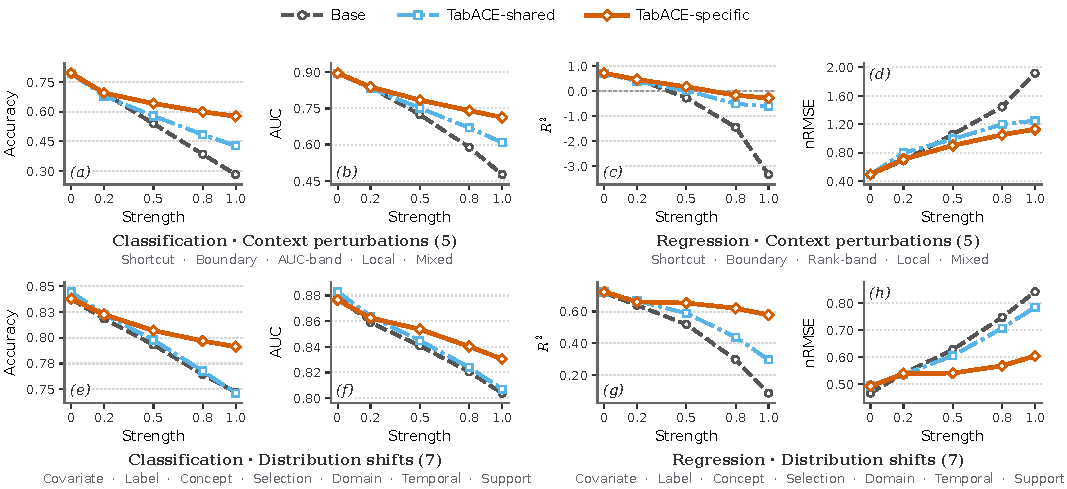
\includegraphics[width=\textwidth]{figures/tabace_limix_2m_strength_summary.pdf}
  \caption{LimiX-2M results across shift strength. Rows aggregate the five
  context perturbations and seven distribution shifts; columns report
  Accuracy, AUC, $R^2$, and nRMSE (lower is better).}
  \label{fig:limix-strength-summary}
\end{figure}

\begin{figure}[H]
  \centering
  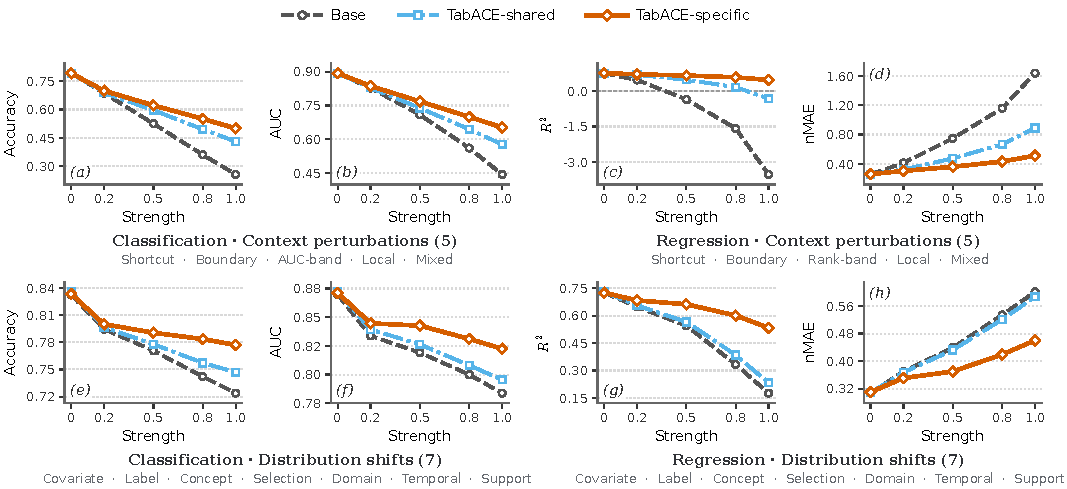
\includegraphics[width=\textwidth]{figures/tabace_tabpfn_v3_strength_summary.pdf}
  \caption{TabPFN-v3 results across shift strength. Rows aggregate the five
  context perturbations and seven distribution shifts; columns report
  Accuracy, AUC, $R^2$, and nMAE (lower is better).}
  \label{fig:tabpfn-strength-summary}
\end{figure}

\begin{figure}[H]
  \centering
  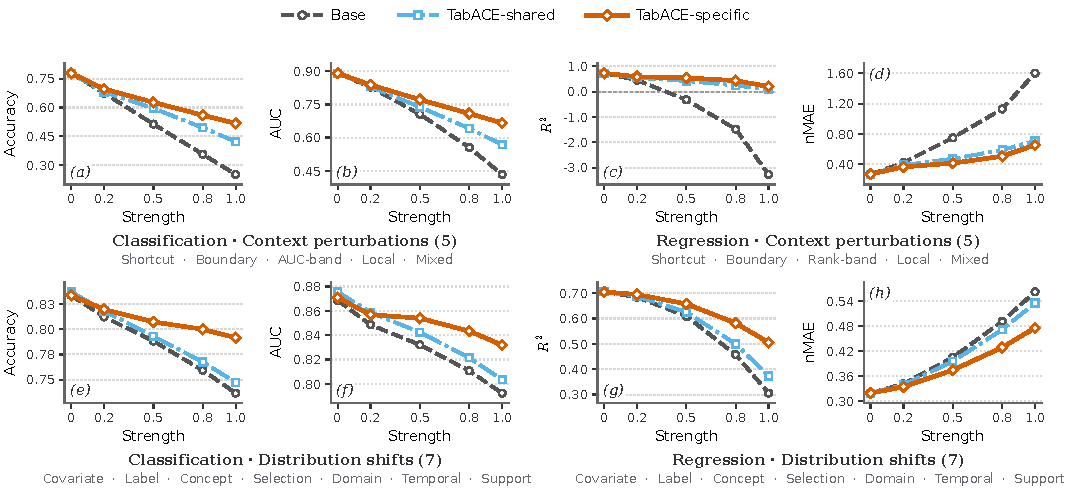
\includegraphics[width=\textwidth]{figures/tabace_tabdpt_v1_2_strength_summary.pdf}
  \caption{TabDPT v1.2 results across shift strength. Rows aggregate the five
  context perturbations and seven distribution shifts; columns report
  Accuracy, AUC, $R^2$, and nMAE (lower is better).}
  \label{fig:tabdpt-strength-summary}
\end{figure}

\FloatBarrier
\section{Ablation Studies}
\label{app:supplemental_ablations}

The ablations use a five-context Shared reference bank selected on each
outer-training fold. The context-budget study evaluates nested prefixes, while
the remaining studies keep all five contexts fixed. This design isolates the
effects of context count, aggregation, and formula components from context
reselection.

\subsection{Context Budget}
\label{app:context-budget}

We vary the context budget from $R=1$ to $R=5$ while holding construction and
aggregation fixed.  The single-context setting trails Base, after which all
six metrics improve monotonically and $R=5$ exceeds Base throughout.  This
trend is consistent with the complementarity analysis in
Section~\ref{sec:theory}: added contexts can cover previously unrepaired queries.

\begin{figure}[H]
  \centering
  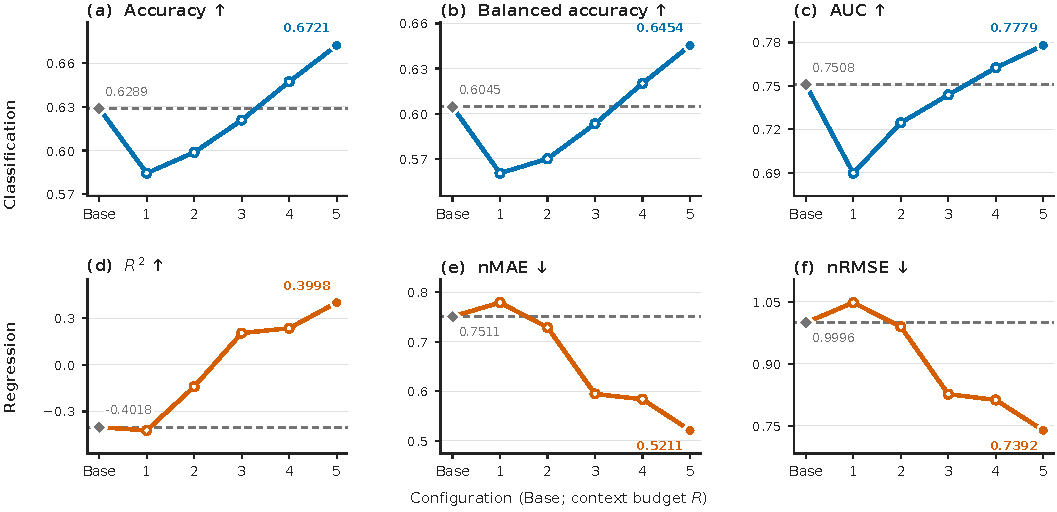
\includegraphics[width=\textwidth]{figures/tabace_context_count_ablation.pdf}
  \caption{Context-count ablation over four nonzero strengths. Each curve
  starts from Base and continues through $R=1,\ldots,5$; dashed horizontal
  lines mark the Base level. The five-perturbation and seven-shift tracks
  receive equal macro weight. With only a few contexts, shift coverage is
  limited. Performance improves as complementary contexts are added, and
  $R=5$ outperforms Base on all six metrics. Arrows indicate the preferred
  direction.}
  \label{fig:context-count}
\end{figure}

\subsection{Aggregation Rule}
\label{app:aggregation-rule}

Using the same five-context bank, we compare mean, median, trimmed-mean, and
out-of-fold weighted aggregation while keeping context count and membership
fixed. For classification, the coordinate-wise median and the mean after
discarding the largest and smallest of five values per class are renormalized
to the probability simplex; regression applies the same operators to scalar
predictions. These context-only variants replace the entire aggregation rule,
so none uses $Q_i$, $S_i$, or the Base gate. The out-of-fold weighted rule attains the highest classification
Accuracy and lowest regression nRMSE, showing the benefit of source-learned
reliability weights over unweighted statistical aggregation for this bank.

\begin{figure}[H]
  \centering
  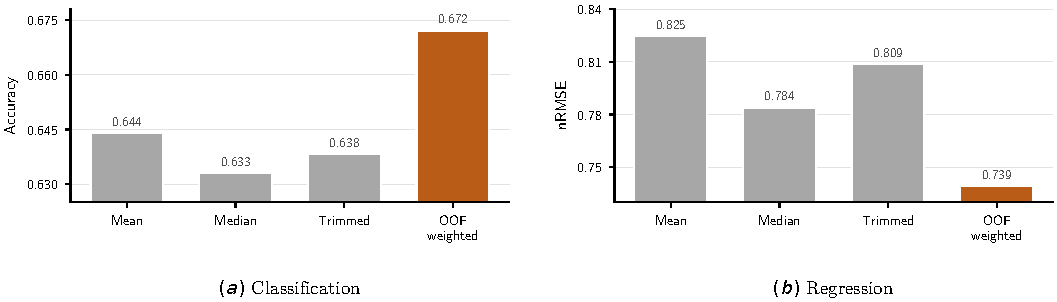
\includegraphics[width=\textwidth]{figures/tabace_aggregation_ablation.pdf}
  \caption{Aggregation-rule ablation at $R=5$, equally weighting the
  five-perturbation and seven-shift tracks. Panels compare classification
  Accuracy and regression nRMSE.}
  \label{fig:aggregation-ablation}
\end{figure}

\subsection{Fixed-Bank Component Ablation}
\label{app:fixed-bank-formula-diagnostic}

Within this diagnostic configuration, we hold each fold-specific five-context
bank fixed and remove one component at a time. All aggregation and gate
parameters are selected on the corresponding
outer-training folds, and outer-test labels are used only for evaluation. We
evaluate five ablations:
\emph{w/o Confidence} sets $\eta_Q=0$ while retaining $Q_i$ in $E_i$;
\emph{w/o Agreement} sets $\eta_S=0$
\textcolor{revisionblue}{while retaining $S_i$ in $E_i$}; \emph{Uniform Prior} sets
$\pi_r=1/R$; \emph{w/o Base Gate} sets $U_i=1$; \emph{w/o context Gate}
sets $E_i=1$. \emph{w/o Confidence} applies to classification, whose formula
includes $Q_i$. The four nonzero strengths are averaged within the
five-perturbation and seven-shift tracks before giving the tracks equal weight.
\textcolor{revisionblue}{The confidence and agreement removals are
weighting-term ablations: they remove the corresponding branch-weight factor,
while retaining the remaining evidence and gate definitions.}

\begin{figure}[H]
  \centering
  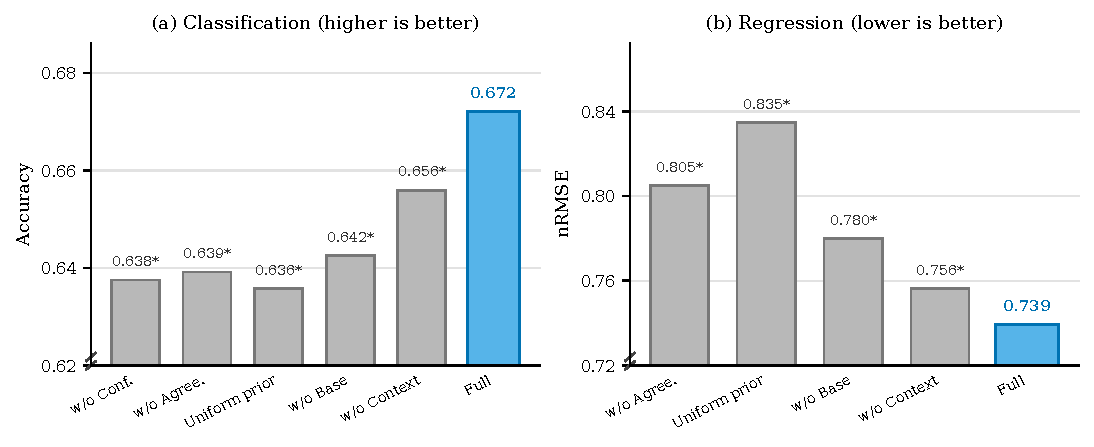
\includegraphics[width=\textwidth]{figures/tabace_k5_formula_diagnostic.pdf}
  \caption{Component ablation for classification and regression. Higher
  Accuracy and lower nRMSE are better. Gray bars remove one component from the
  fixed-bank reference, shown by the final blue bar. Values are printed above
  each bar, and asterisks mark Holm-corrected paired sign-flip $p<0.05$
  relative to this reference. Break marks indicate truncated vertical axes.}
  \label{fig:k5-formula-diagnostic}
\end{figure}

The fixed-bank reference reaches 0.672 Accuracy and 0.739 nRMSE. Removing
confidence, agreement,
the learned prior, Base gating, or context gating reduces classification
Accuracy to 0.638, 0.639, 0.636, 0.642, and 0.656, respectively. For
regression, removing agreement, the learned prior, Base gating, or context
gating increases nRMSE to 0.805, 0.835, 0.780, and 0.756. Every displayed
difference is significant after Holm correction, with the largest degradation
arising from the learned context prior on both tasks.

\subsection{Gate Behavior across Evidence Bins}
\label{app:gate-bin-analysis}

We partition 752,144 query predictions into task-wise tertiles of Base
unreliability $U_i$ and context evidence $E_i$. Each cell reports the mean
interpolation weight and loss gain over Base, together with the fraction of
material modifications ($\alpha_i\geq0.5$) and their worsening rate.

\begin{figure}[H]
  \centering
  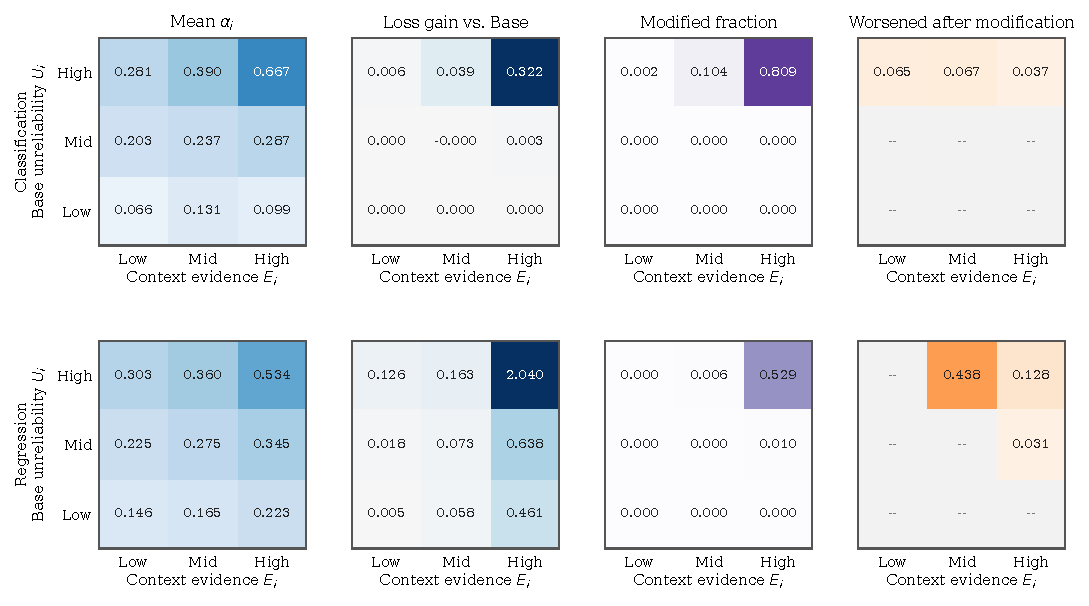
\includegraphics[width=0.78\textwidth]{figures/tabace_gate_bin_analysis.pdf}
  \caption{Gate behavior across Base-unreliability ($U_i$) and context-evidence
  ($E_i$) tertiles. Positive gain indicates improvement; gray cells contain no
  material modifications. In the high-$U_i$/high-$E_i$ bin,
  classification/regression attain interpolation weights of 0.667/0.534,
  modification rates of 0.809/0.529, loss gains of 0.322/2.040, and worsening
  rates of 0.037/0.128; low/low loss gains are 0.000/0.005.}
  \label{fig:gate-bin-analysis}
\end{figure}

In the regression high-$U_i$/mid-$E_i$ cell, only $0.6\%$ of queries receive
a material update; their conditional worsening rate is $43.8\%$, while the
cell-level mean loss gain remains positive at $0.163$.

\FloatBarrier
\endgroup

% Generated from revision_data/rebuttal_tables.json and author-provided response tables.
\clearpage
\begingroup
\providecolor{revisionblue}{RGB}{25,55,135}
\color{revisionblue}
\section{Additional Experiments and Clarifications during Discussion}
\label{app:rebuttal-additions}

This section collects the additional evaluations discussed in the author
responses. Newly added material is shown in blue to help locate revisions.
These supplementary evaluations complement the original results; configuration
adaptations, development-task changes, and repeated-run statistics are identified
where applicable rather than replacing the original benchmark definitions.

\subsection{Ensemble Comparisons}
\label{app:revision-ensembles}

Tables~\ref{tab:revision-tabicl-cls}--\ref{tab:revision-tabpfn-reg} give
the supplementary ensemble comparisons. Classification cells report
Accuracy/AUROC and regression cells report $R^2$/nRMSE. Each robustness block
averages its nonzero strengths over the five perturbation or seven shift families.
Native-6 uses the backbone's native ensemble; Random-6 averages six sampled
contexts. GES selects members greedily; convex and log-linear stacking learn
fixed fusion rules. Median, trimmed-mean, and IQR variants provide robust
aggregation or uncertainty-based selection controls. DENSE follows demonstration
ensembling~\citep{khalifa2023dense}; PHE and RF-PFN follow the TabPFN
ensemble components~\citep{hollmann2025tabpfn}. OligoICP uses low-IQR member
selection and averaging~\citep{revision_li2025oligo}.

The suffix ``6'' denotes six deployed predictions; Shared uses Base and five
alternatives. OligoICP $60\!\rightarrow\!6$ and $400\!\rightarrow\!40$
denote candidate/deployed counts. The latter has a larger deployment budget and
is reported separately from six-member comparisons. Candidate generation and
selection are additional preparation costs, not counted as deployed predictions.
An asterisk marks a component-level or budget-adapted implementation; a dagger
marks an adapted supplementary configuration, not necessarily backbone fine-tuning.

\begin{table}[H]
\centering\footnotesize
\color{revisionblue}
\setlength{\tabcolsep}{4pt}
\renewcommand{\arraystretch}{1.12}
\caption{TabICL-v2 classification ensemble comparison (Accuracy/AUROC).}
\label{tab:revision-tabicl-cls}
\resizebox{\linewidth}{!}{%
\begin{tabular}{@{}lrrr@{}}
\toprule
Method & Clean & Five perturbations & Seven shifts \\
\midrule
TabICL-v2 Base & 0.804 / 0.901 & 0.494 / 0.676 & 0.763 / 0.826 \\
Native-6 & 0.803 / 0.901 & 0.507 / 0.683 & 0.763 / 0.825 \\
Random-6 & 0.800 / 0.897 & 0.523 / 0.696 & 0.764 / 0.828 \\
DENSE-6 & 0.798 / 0.897 & 0.531 / 0.695 & 0.764 / 0.826 \\
GES-6 & 0.801 / 0.899 & 0.539 / 0.694 & 0.765 / 0.827 \\
Convex Stacking-6 & 0.800 / 0.898 & 0.559 / 0.704 & 0.766 / 0.827 \\
Log-linear Stacking-6 & 0.803 / 0.901 & 0.535 / 0.692 & 0.763 / 0.824 \\
TabFM feature-view NNLS-6 & 0.805 / 0.901 & 0.506 / 0.672 & 0.767 / 0.827 \\
Divide-and-conquer & 0.805 / 0.902 & 0.503 / 0.672 & 0.763 / 0.825 \\
Shared & 0.804 / 0.901 & \textbf{0.575 / 0.720} & \textbf{0.772 / 0.831} \\
\bottomrule
\end{tabular}}
\end{table}


\begin{table}[H]
\centering\footnotesize
\color{revisionblue}
\setlength{\tabcolsep}{4pt}
\renewcommand{\arraystretch}{1.12}
\caption{TabICL-v2 regression ensemble comparison ($R^2$/nRMSE).}
\label{tab:revision-tabicl-reg}
\resizebox{\linewidth}{!}{%
\begin{tabular}{@{}lrrr@{}}
\toprule
Method & Clean & Five perturbations & Seven shifts \\
\midrule
TabICL-v2 Base & 0.739 / 0.476 & -1.077 / 1.270 & 0.273 / 0.730 \\
Native-6 & 0.740 / 0.487 & -0.597 / 1.145 & 0.287 / 0.721 \\
Random-6 & 0.742 / 0.505 & -0.397 / 1.089 & 0.351 / 0.702 \\
GES-6 & 0.731 / 0.501 & -0.434 / 1.103 & 0.397 / 0.684 \\
Convex Stacking-6 & 0.733 / 0.499 & -0.446 / 1.104 & 0.401 / 0.682 \\
Ridge Stacking-6 & 0.732 / 0.500 & -0.457 / 1.111 & 0.416 / 0.683 \\
Median-6\textsuperscript{\(\dagger\)} & 0.734 / 0.496 & -0.505 / 1.121 & 0.421 / 0.675 \\
Feature Mean-6 & 0.734 / 0.496 & -0.461 / 1.109 & 0.421 / 0.677 \\
Trimmed Mean-6 & 0.735 / 0.492 & -0.483 / 1.114 & 0.419 / 0.676 \\
IQR-selection & 0.728 / 0.501 & -0.446 / 1.102 & 0.353 / 0.702 \\
Shared & 0.738 / 0.478 & \textbf{0.363 / 0.783} & \textbf{0.467 / 0.659} \\
\bottomrule
\end{tabular}}
\end{table}


\begin{table}[H]
\centering\footnotesize
\color{revisionblue}
\setlength{\tabcolsep}{4pt}
\renewcommand{\arraystretch}{1.12}
\caption{TabPFN classification ensemble comparison (Accuracy/AUROC).}
\label{tab:revision-tabpfn-cls}
\resizebox{\linewidth}{!}{%
\begin{tabular}{@{}lrrr@{}}
\toprule
Method & Clean & Five perturbations & Seven shifts \\
\midrule
TabPFN Base & 0.793 / 0.893 & 0.457 / 0.636 & 0.758 / 0.809 \\
Native-6 & 0.799 / 0.899 & 0.467 / 0.637 & 0.766 / 0.814 \\
PHE-6 & 0.802 / 0.900 & 0.464 / 0.626 & 0.763 / 0.816 \\
RF-PFN-6 & 0.806 / 0.901 & 0.470 / 0.629 & 0.760 / 0.817 \\
MICP component* & 0.783 / 0.892 & 0.461 / 0.626 & 0.751 / 0.816 \\
Shared & 0.792 / 0.893 & \textbf{0.553 / 0.697} & \textbf{0.770} / 0.817 \\
\bottomrule
\end{tabular}}
\end{table}


\begin{table}[H]
\centering\footnotesize
\color{revisionblue}
\setlength{\tabcolsep}{4pt}
\renewcommand{\arraystretch}{1.12}
\caption{TabPFN regression ensemble comparison ($R^2$/nRMSE).}
\label{tab:revision-tabpfn-reg}
\resizebox{\linewidth}{!}{%
\begin{tabular}{@{}lrrr@{}}
\toprule
Method & Clean & Five perturbations & Seven shifts \\
\midrule
TabPFN Base & 0.739 / 0.476 & -1.253 / 1.313 & 0.426 / 0.669 \\
Native-6\textsuperscript{\(\dagger\)} & 0.737 / 0.508 & -0.405 / 1.116 & 0.444 / 0.640 \\
PHE-6\textsuperscript{\(\dagger\)} & 0.728 / 0.516 & -0.387 / 1.111 & 0.424 / 0.659 \\
RF-PFN-6\textsuperscript{\(\dagger\)} & 0.737 / 0.509 & -0.400 / 1.116 & 0.444 / 0.660 \\
OligoICP 60\(\rightarrow\)6*\textsuperscript{\(\dagger\)} & 0.703 / 0.549 & -0.370 / 1.120 & 0.333 / 0.703 \\
OligoICP 400\(\rightarrow\)40*\textsuperscript{\(\dagger\)} & 0.697 / 0.549 & -0.325 / 1.104 & 0.355 / 0.695 \\
Shared & 0.739 / 0.480 & \textbf{0.237 / 0.834} & \textbf{0.460} / 0.656 \\
\bottomrule
\end{tabular}}
\end{table}



\subsection{Larger Context Budgets}
\label{app:revision-large-context}
We evaluate TabICL-v2 with row caps of 1,024, 4,096, and 8,192 for Base,
Shared, and Specific. The sample counts are 72 classification/35 regression
datasets for clean and perturbed evaluation, and 35/33 for shifts.
These are supplementary calibrated development-benchmark evaluations; the
regression clean and perturbed tasks include semisynthetic reconstruction.
For the regression recovery protocol, the original 256-row perturbed core is
retained and added context rows come from clean training data. Thus these
recovery results include the contribution of extra clean evidence as the budget
increases, rather than keeping the contamination fraction fixed.
Tables~\ref{tab:revision-large-cls} and~\ref{tab:revision-large-reg}
report the additional results. The compact 256-row budget is also examined in
TabDPT's inference ablation~\citep{ma2025tabdpt}; it is not its capacity limit.

\begin{table}[H]
\centering\footnotesize
\color{revisionblue}
\setlength{\tabcolsep}{4pt}
\renewcommand{\arraystretch}{1.12}
\caption{Larger-context classification (Accuracy/AUROC); columns cover 72/72/35 datasets.}
\label{tab:revision-large-cls}
\resizebox{\linewidth}{!}{%
\begin{tabular}{@{}lrrrr@{}}
\toprule
Context cap & Method & Clean & Five perturbations & Seven shifts \\
\midrule
1024 & Base & 0.8254 / 0.9218 & 0.5332 / 0.7015 & 0.7635 / 0.8474 \\
1024 & Shared & 0.8268 / 0.9223 & 0.6586 / 0.8044 & 0.7762 / 0.8661 \\
1024 & Specific & \textbf{0.8289 / 0.9229} & \textbf{0.6917 / 0.8374} & \textbf{0.8047 / 0.8767} \\
4096 & Base & 0.8381 / 0.9304 & 0.5446 / 0.7105 & 0.7607 / 0.8554 \\
4096 & Shared & 0.8402 / 0.9306 & 0.6790 / 0.8116 & 0.7738 / 0.8724 \\
4096 & Specific & \textbf{0.8436 / 0.9308} & \textbf{0.7071 / 0.8433} & \textbf{0.7982 / 0.8806} \\
8192 & Base & 0.8416 / 0.9314 & 0.5469 / 0.7107 & 0.7625 / 0.8576 \\
8192 & Shared & 0.8433 / 0.9315 & 0.6814 / 0.8124 & 0.7746 / 0.8734 \\
8192 & Specific & \textbf{0.8456 / 0.9316} & \textbf{0.7115 / 0.8440} & \textbf{0.8042 / 0.8824} \\
\bottomrule
\end{tabular}}
\end{table}


\begin{table}[H]
\centering\footnotesize
\color{revisionblue}
\setlength{\tabcolsep}{4pt}
\renewcommand{\arraystretch}{1.12}
\caption{Larger-context regression ($R^2$/nRMSE); columns cover 35/35/33 datasets.}
\label{tab:revision-large-reg}
\resizebox{\linewidth}{!}{%
\begin{tabular}{@{}lrrrr@{}}
\toprule
Context cap & Method & Clean & Five perturbations & Seven shifts \\
\midrule
1024 & Base & 0.7557 / 0.4680 & -1.0547 / 1.2598 & 0.2891 / 0.6659 \\
1024 & Shared & 0.7570 / 0.4662 & 0.4779 / 0.6803 & 0.5816 / 0.5533 \\
1024 & Specific & \textbf{0.7573 / 0.4633} & \textbf{0.5968 / 0.6051} & \textbf{0.7322 / 0.4569} \\
4096 & Base & 0.7590 / 0.4647 & -1.0380 / 1.2560 & 0.3265 / 0.6379 \\
4096 & Shared & 0.7599 / 0.4627 & 0.4800 / 0.6793 & 0.5980 / 0.5325 \\
4096 & Specific & \textbf{0.7604 / 0.4622} & \textbf{0.5985 / 0.6040} & \textbf{0.7512 / 0.4306} \\
8192 & Base & 0.7596 / 0.4642 & -1.0317 / 1.2545 & 0.3287 / 0.6310 \\
8192 & Shared & 0.7603 / 0.4623 & 0.4809 / 0.6790 & 0.5864 / 0.5328 \\
8192 & Specific & \textbf{0.7609 / 0.4621} & \textbf{0.5989 / 0.6038} & \textbf{0.7649 / 0.4109} \\
\bottomrule
\end{tabular}}
\end{table}



\subsection{Calibration Coverage and Constructor Matching}
\label{app:revision-matching}
The $2\times2$ Shortcut experiment independently varies whether calibration
includes Shortcut and whether the matched feature-removal constructor is present.
B/D exclude Shortcut from policy calibration; C/D use nonmatching constructions.
The comparisons use the same available supervision. This diagnostic separately
tests calibration transfer and the need for a matched constructor.
Problem-aware construction is useful when domain knowledge is available: SPN
constructs strategic contexts for post-manipulation inputs~\citep{lv2026strategic}.
Shared instead operates without a mechanism identifier.

\begin{table}[H]
\centering\footnotesize
\color{revisionblue}
\setlength{\tabcolsep}{4pt}
\renewcommand{\arraystretch}{1.12}
\caption{Shortcut calibration/constructor-matching ablation.}
\label{tab:revision-matching}
\resizebox{\linewidth}{!}{%
\begin{tabular}{@{}lrrrr@{}}
\toprule
Configuration & Shortcut in calibration & Matched constructor & Acc $\uparrow$ & AUC $\uparrow$ \\
\midrule
Base & --- & --- & 0.51719 & 0.65690 \\
A & Yes & Yes & \textbf{0.74394} & \textbf{0.87909} \\
B & No & Yes & 0.70777 & 0.85370 \\
C & Yes & No & 0.71187 & 0.85757 \\
D & No & No & 0.69333 & 0.84662 \\
\bottomrule
\end{tabular}}
\end{table}



\subsection{Unseen Perturbations and Distribution Shifts}
\label{app:revision-unseen}
All six mechanisms below are excluded from policy calibration and have no
dedicated matching constructors added to the Shared bank. Strengths are
$s\in\{0.2,0.5,0.8,1.0\}$; results average strengths and datasets.
Use source-feature median $m$ and IQR $a$ (falling back to the standard
deviation for zero IQR) as location and scale. Heavy-tailed corruption selects
numeric cells with probability $0.1s$ and adds
$2a\,\operatorname{clip}(t_2,-20,20)$, with $t_2$ Student-$t$ noise.
Column misalignment independently permutes approximately half of nonconstant
columns within approximately $0.5s$ of source rows. Quantization rounds numeric
source features to a grid with step $sa$.

For sensor transformation let $z=(x-m)/a$ and set
$\widetilde x=m+a\operatorname{sign}(z)\log(1+s|z|)/s$.
Rotation randomly pairs numeric features and rotates standardized pairs by
$s\pi/4$ before restoring scale. These two maps act on target-query features for
classification and source-context features for regression. Interaction-dependent
sampling selects up to eight nonconstant feature pairs, computes the average
product of their standardized, $\tanh$-compressed values $g_i$, and resamples
complete source rows with $w_i\propto\exp(3s g_i)$. Associated labels travel
with each row; target labels are not used to generate these changes.

\begin{table}[H]
\centering\footnotesize
\color{revisionblue}
\setlength{\tabcolsep}{4pt}
\renewcommand{\arraystretch}{1.12}
\caption{Classification under unseen mechanisms (Accuracy/AUROC).}
\label{tab:revision-unseen-cls}
\resizebox{\linewidth}{!}{%
\begin{tabular}{@{}lrrr@{}}
\toprule
Unseen mechanism & Datasets & Base & Shared \\
\midrule
Heavy-tailed noise & 64 & 0.7875 / 0.8932 & \textbf{0.8176 / 0.9068} \\
Column misalignment & 72 & 0.7824 / 0.8920 & \textbf{0.8186 / 0.9100} \\
Feature quantization & 64 & 0.7070 / 0.8782 & \textbf{0.7576 / 0.8902} \\
Feature rotation & 31 & 0.7609 / 0.8217 & \textbf{0.7861 / 0.8420} \\
Nonlinear sensor transformations & 32 & 0.8002 / 0.8524 & \textbf{0.8208 / 0.8600} \\
Interaction-dependent sampling & 35 & 0.8214 / 0.8676 & \textbf{0.8288 / 0.8779} \\
\bottomrule
\end{tabular}}
\end{table}


\begin{table}[H]
\centering\footnotesize
\color{revisionblue}
\setlength{\tabcolsep}{4pt}
\renewcommand{\arraystretch}{1.12}
\caption{Regression under unseen mechanisms ($R^2$/nRMSE).}
\label{tab:revision-unseen-reg}
\resizebox{\linewidth}{!}{%
\begin{tabular}{@{}lrrr@{}}
\toprule
Unseen mechanism & Datasets & Base & Shared \\
\midrule
Heavy-tailed noise & 35 & 0.6380 / 0.5417 & \textbf{0.6757 / 0.5161} \\
Column misalignment & 35 & 0.6179 / 0.5591 & \textbf{0.6751 / 0.5170} \\
Feature quantization & 35 & 0.3743 / 0.7070 & \textbf{0.5023 / 0.6452} \\
Feature rotation & 31 & 0.3375 / 0.7527 & \textbf{0.4663 / 0.6810} \\
Nonlinear sensor transformations & 33 & 0.1009 / 0.8235 & \textbf{0.4413 / 0.6665} \\
Interaction-dependent sampling & 33 & 0.6487 / 0.5350 & \textbf{0.6860 / 0.5042} \\
\bottomrule
\end{tabular}}
\end{table}



\subsection{Natural Shifts and Repeated Runs}
\label{app:revision-natural}
\subsubsection{Folktables Context Lists}
\label{app:revision-folktables-contexts}
Geographic transfer uses California to Michigan (2018); temporal transfer uses
California 2014 to 2018, on Employment, Income, and TravelTime. Specific uses
source-to-target domain-shift contexts: the five Shared alternatives plus three
additional constructions, each capped at 512 rows (six/nine predictions including
Base). The following is the deployed list for this supplementary Folktables study,
not a uniform branch-count claim for every main-benchmark family.
For this deployed list, $R_{\mathrm{Shared}}=5$ and
$R_{\mathrm{Specific}}=8$; including Base gives
$N_{\mathrm{Shared}}=6$ and $N_{\mathrm{Specific}}=9$ predictions per query.
The five shared types and three additional Specific types are enumerated below.

Let $z_i$ denote robustly standardized source features, $d_i$ the mean squared distance to the ten nearest target examples, $o_i=\operatorname{mean}_j z_{ij}^2$, and $\delta_i=1-\max_c\frac1{10}\sum_{k\in N_{10}(i)}\mathbf1[y_k=c]$ the source-neighborhood label-conflict score. Unless stated otherwise, we retain the lowest-scoring source rows and sample without replacement.

\begin{itemize}

\item \textbf{Target neighborhood (Shared/Specific):} Form target anchors $A_Q$ from the coordinate-wise 10th, 30th, 50th, 70th, and 90th percentiles; rank by $s_i=\min_{a\in A_Q}\|z_i-a\|_2^2$ and retain 80\%.

\item \textbf{Representative samples (Shared/Specific):} Rank by $s_i=d_i+0.35o_i$ and retain 70\%.

\item \textbf{Local stability (Shared/Specific):} Rank by $s_i=\delta_i+0.10d_i$ and retain 80\%.

\item \textbf{Feature subspace (Shared/Specific):} Remove $j^*=\arg\max_j|\operatorname{corr}(X_j,y)|$ from both context and query, then sample source rows.

\item \textbf{Low conflict (Shared/Specific):} Rank by $s_i=\delta_i+0.20o_i$ and retain 75\%.

\item \textbf{Target-matched bootstrap (Specific):} Standardize continuous features and one-hot encode categorical features; sample with replacement using $w_i\propto\exp(-d_i^{\mathrm{mix}}/h)$, where $d_i^{\mathrm{mix}}$ is the ten-neighbor target distance and $h$ is its positive median, preserving class coverage.

\item \textbf{Density-ratio bootstrap (Specific):} Fit a logistic domain classifier $g(x)$ and sample with replacement using $w_i\propto[\min\{\frac{g(x_i)}{1-g(x_i)}\frac{n_s}{n_t},10\}]^{1/2}$, preserving class coverage; $n_s,n_t$ are source and target sample counts.

\item \textbf{Continuous-feature alignment (Specific):} For prespecified continuous features, apply $T(x)=0.5x+0.5[(x-m_s)s_t/s_s+m_t]$, where $m$ is the median and $s=\max(\mathrm{IQR},1)$. Sample source rows without replacement, retaining source labels and categorical features.

\end{itemize}


\subsubsection{Folktables Accuracy Comparisons}
\label{app:revision-folktables-comparison}
DistPFN uses the TabICL-v2 backbone~\citep{lee2026distpfn}; Drift-Resilient
TabPFN uses its own model~\citep{helli2024drifttabpfn}. Table~\ref{tab:revision-folktables}
reports the accuracy comparisons and baseline dispersions. The separate
repeated-run configuration below has its own statistics.

\begin{table}[H]
\centering\footnotesize
\color{revisionblue}
\setlength{\tabcolsep}{4pt}
\renewcommand{\arraystretch}{1.12}
\caption{Folktables accuracy; Geog. and Temp. denote geographic and temporal transfer.}
\label{tab:revision-folktables}
\resizebox{\linewidth}{!}{%
\begin{tabular}{@{}lrrrrrrr@{}}
\toprule
Shift & Task & Domain & Base & DistPFN & Drift-res. & Shared & Specific \\
\midrule
Geog. & Employment & ID & 0.7922 & 0.7892 \(\pm\) 0.0030 & 0.7885 \(\pm\) 0.0071 & \textbf{0.7952} & \textbf{0.8089} \\
Geog. & Employment & OOD & 0.8043 & 0.8034 \(\pm\) 0.0033 & 0.8022 \(\pm\) 0.0067 & \textbf{0.8106} & \textbf{0.8245} \\
Geog. & Income & ID & 0.7888 & 0.7930 \(\pm\) 0.0100 & 0.7856 \(\pm\) 0.0147 & \textbf{0.8118} & \textbf{0.8201} \\
Geog. & Income & OOD & 0.7655 & 0.7768 \(\pm\) 0.0288 & 0.7733 \(\pm\) 0.0209 & \textbf{0.7823} & \textbf{0.7914} \\
Geog. & TravelTime & ID & 0.5912 & 0.5731 \(\pm\) 0.0253 & 0.5723 \(\pm\) 0.0252 & \textbf{0.6225} & \textbf{0.6569} \\
Geog. & TravelTime & OOD & 0.5472 & 0.5802 \(\pm\) 0.0071 & 0.5667 \(\pm\) 0.0338 & \textbf{0.5818} & \textbf{0.6012} \\
Temp. & Employment & ID & 0.7704 & 0.7770 \(\pm\) 0.0043 & 0.7699 \(\pm\) 0.0095 & \textbf{0.7861} & \textbf{0.7994} \\
Temp. & Employment & OOD & 0.7847 & 0.7804 \(\pm\) 0.0090 & 0.7742 \(\pm\) 0.0140 & \textbf{0.7922} & \textbf{0.8030} \\
Temp. & Income & ID & 0.7926 & 0.8009 \(\pm\) 0.0050 & 0.8010 \(\pm\) 0.0055 & \textbf{0.8126} & \textbf{0.8240} \\
Temp. & Income & OOD & 0.7844 & 0.7894 \(\pm\) 0.0040 & 0.7867 \(\pm\) 0.0054 & \textbf{0.8000} & \textbf{0.8106} \\
Temp. & TravelTime & ID & 0.5951 & 0.5937 \(\pm\) 0.0235 & 0.5956 \(\pm\) 0.0145 & \textbf{0.6237} & \textbf{0.6526} \\
Temp. & TravelTime & OOD & 0.5908 & 0.5731 \(\pm\) 0.0309 & 0.5692 \(\pm\) 0.0179 & \textbf{0.6045} & \textbf{0.6350} \\
\bottomrule
\end{tabular}}
\end{table}



\subsubsection{Seed Variability}
\label{app:revision-folktables-variance}
For a separate source-supervised adapted configuration, repeat seeds 0--4 with
fixed data partitions and hyperparameters. Table~\ref{tab:revision-folktables-variance}
reports sample standard deviation and sample variance
$s^2=\frac14\sum_{k=0}^4(a_k-\bar a)^2$. These quantify context sampling,
model randomness, and adaptation under the fixed split; they are not attached
to the different point estimates in Table~\ref{tab:revision-folktables}.

\begin{table}[H]
\centering\footnotesize
\color{revisionblue}
\setlength{\tabcolsep}{4pt}
\renewcommand{\arraystretch}{1.12}
\caption{Five-seed Folktables variability: $\pm$ sample standard deviation (sample variance), Accuracy scale.}
\label{tab:revision-folktables-variance}
\resizebox{\linewidth}{!}{%
\begin{tabular}{@{}lrrrrr@{}}
\toprule
Shift & Task & Domain & Base & Shared & Specific \\
\midrule
Geog. & Employment & ID & \(\pm\)0.0031 (9.397e-06) & \(\pm\)0.0031 (9.827e-06) & \(\pm\)0.0042 (1.737e-05) \\
Geog. & Employment & OOD & \(\pm\)0.0044 (1.934e-05) & \(\pm\)0.0047 (2.164e-05) & \(\pm\)0.0040 (1.602e-05) \\
Geog. & Income & ID & \(\pm\)0.0099 (9.749e-05) & \(\pm\)0.0020 (3.942e-06) & \(\pm\)0.0003 (8.800e-08) \\
Geog. & Income & OOD & \(\pm\)0.0222 (4.921e-04) & \(\pm\)0.0063 (4.016e-05) & \(\pm\)0.0029 (8.404e-06) \\
Geog. & TravelTime & ID & \(\pm\)0.0222 (4.945e-04) & \(\pm\)0.0212 (4.498e-04) & \(\pm\)0.0101 (1.029e-04) \\
Geog. & TravelTime & OOD & \(\pm\)0.0304 (9.251e-04) & \(\pm\)0.0349 (1.220e-03) & \(\pm\)0.0062 (3.817e-05) \\
Temp. & Employment & ID & \(\pm\)0.0040 (1.632e-05) & \(\pm\)0.0028 (7.777e-06) & \(\pm\)0.0031 (9.693e-06) \\
Temp. & Employment & OOD & \(\pm\)0.0084 (7.110e-05) & \(\pm\)0.0053 (2.851e-05) & \(\pm\)0.0015 (2.223e-06) \\
Temp. & Income & ID & \(\pm\)0.0045 (1.985e-05) & \(\pm\)0.0042 (1.744e-05) & \(\pm\)0.0011 (1.307e-06) \\
Temp. & Income & OOD & \(\pm\)0.0033 (1.099e-05) & \(\pm\)0.0027 (7.438e-06) & \(\pm\)0.0031 (9.633e-06) \\
Temp. & TravelTime & ID & \(\pm\)0.0236 (5.579e-04) & \(\pm\)0.0076 (5.840e-05) & \(\pm\)0.0088 (7.697e-05) \\
Temp. & TravelTime & OOD & \(\pm\)0.0309 (9.554e-04) & \(\pm\)0.0126 (1.594e-04) & \(\pm\)0.0114 (1.304e-04) \\
\bottomrule
\end{tabular}}
\end{table}



\subsubsection{Additional Clinical Shifts}
\label{app:revision-medical}
PhysioNet Sepsis 2019 uses bidirectional hospital-system A/B transfer. UCI
Diabetes 130-US Hospitals uses non-emergency-room to emergency-room admission
source transfer. ID and OOD denote held-out source and target domains.
The table reports the case--control component evaluation with balanced classes
(1:1); this changes prevalence relative to the natural clinical population.

\begin{table}[H]
\centering\footnotesize
\color{revisionblue}
\setlength{\tabcolsep}{4pt}
\renewcommand{\arraystretch}{1.12}
\caption{Clinical domain-shift component evaluation (Accuracy; 1:1 case--control).}
\label{tab:revision-medical}
\resizebox{\linewidth}{!}{%
\begin{tabular}{@{}lrrrrr@{}}
\toprule
Dataset & Task & Domain & Base & Shared & Specific \\
\midrule
Sepsis 2019 & Sepsis A $\rightarrow$ B & ID & 70.20\% & \textbf{70.71\%} & \textbf{71.72\%} \\
Sepsis 2019 & Sepsis A $\rightarrow$ B & OOD & 61.59\% & \textbf{62.14\%} & \textbf{63.04\%} \\
Sepsis 2019 & Sepsis B $\rightarrow$ A & ID & 76.19\% & \textbf{77.38\%} & \textbf{78.57\%} \\
Sepsis 2019 & Sepsis B $\rightarrow$ A & OOD & 63.79\% & \textbf{64.60\%} & \textbf{64.91\%} \\
Diabetes 130-US & Readmission & ID & 54.82\% & \textbf{55.26\%} & \textbf{56.87\%} \\
Diabetes 130-US & Readmission & OOD & 57.27\% & \textbf{58.97\%} & \textbf{59.24\%} \\
\bottomrule
\end{tabular}}
\end{table}



\subsection{Robust Backbone Fine-Tuning}
\label{app:revision-finetuning}
FT updates TabICL-v2 on 20\% clean and 80\% corruption-augmented training
episodes at strengths $\{0.2,0.5,0.8,1.0\}$. AdamW updates the last four ICL
blocks and prediction components. Held-out training data select checkpoints;
final evaluation queries do not train or select the models. FT+Shared/Specific
freeze the fine-tuned backbone and apply context fusion at inference.
All compared methods use the same queries within this supplementary benchmark.
In the corrected comparison, context-row budgets are held fixed across the
corruption and shift blocks within each task. Shared/Specific retain their
context-and-fusion adaptation; regression clean and five-perturbation results
include supplementary semisynthetic tasks.

\begin{table}[H]
\centering\footnotesize
\color{revisionblue}
\setlength{\tabcolsep}{4pt}
\renewcommand{\arraystretch}{1.12}
\caption{Corrected fine-tuning and inference-time context adaptation; classification Accuracy/AUROC and regression $R^2$/nRMSE.}
\label{tab:revision-finetuning}
\resizebox{\linewidth}{!}{%
\begin{tabular}{@{}lrrrr@{}}
\toprule
Task & Method & Clean & Five corruptions (avg.) & Seven shifts (avg.) \\
\midrule
Classification & Base & 0.8033 / 0.9007 & 0.4973 / 0.6729 & 0.7634 / 0.8246 \\
Classification & Shared & 0.8048 / 0.9030 & 0.5818 / 0.7253 & 0.7747 / 0.8392 \\
Classification & Specific & 0.8041 / 0.9013 & 0.6132 / 0.7661 & 0.8197 / 0.8576 \\
Classification & FT & 0.7970 / 0.8998 & 0.5399 / 0.6978 & 0.7687 / 0.8301 \\
Classification & FT+Shared & 0.7994 / 0.9019 & 0.5919 / 0.7350 & 0.7846 / 0.8404 \\
Classification & FT+Specific & 0.8018 / 0.9020 & 0.6135 / 0.7706 & 0.8220 / 0.8682 \\
Regression & Base & 0.7425 / 0.4803 & -1.0763 / 1.2685 & 0.2746 / 0.7288 \\
Regression & Shared & 0.7400 / 0.4825 & 0.3637 / 0.7845 & 0.4652 / 0.6564 \\
Regression & Specific & 0.7519 / 0.4710 & 0.4855 / 0.7069 & 0.6531 / 0.5365 \\
Regression & FT & 0.6942 / 0.5275 & 0.3102 / 0.8494 & 0.3897 / 0.6898 \\
Regression & FT+Shared & 0.7178 / 0.5062 & 0.4099 / 0.7297 & 0.5503 / 0.6105 \\
Regression & FT+Specific & 0.7253 / 0.4994 & 0.4401 / 0.7199 & 0.6101 / 0.5693 \\
\bottomrule
\end{tabular}}
\end{table}



The recorded run configuration uses eight RTX 5090 GPUs (32 GB each), one job
per GPU, for 175 dataset--track jobs. Selected-model training averages
41.4 seconds/model; all recorded candidates total 147.8 GPU-minutes. The latter
is summed device time, not elapsed wall-clock time. For context, the original
inference-cost experiment reports median Shared latencies of 872 ms for
classification and 141 ms for regression. Direct inference-time use avoids
backbone optimization; these timing measurements describe distinct stages.

\subsection{Gate Diagnostics and Robustness Extensions}
\label{app:revision-gate}
\subsubsection{High-Confidence Classification Errors}
\label{app:revision-high-confidence}
On the reconstructed five-perturbation benchmark, high-confidence Base errors
(maximum class probability at least 0.9) occupy 2.06--2.44\% of all
query--condition pairs. An extended update-strength estimator adds relative
Base/context confidence, disagreement, and branch consensus; branch aggregation
is unchanged and the added score is calibrated on training folds.

\begin{table}[H]
\centering\footnotesize
\color{revisionblue}
\setlength{\tabcolsep}{4pt}
\renewcommand{\arraystretch}{1.12}
\caption{High-confidence error corrections on reconstructed five-perturbation data (original $\rightarrow$ extended).}
\label{tab:revision-high-confidence}
\resizebox{\linewidth}{!}{%
\begin{tabular}{@{}lrrrr@{}}
\toprule
Backbone & HC errors/all & Correction rate & Corrected & Overall Acc \\
\midrule
TabICL & 2.06\% & 0 \(\rightarrow\) \textbf{17.09\%} & 648 & 67.5532\% \(\rightarrow\) \textbf{67.8380\%} \\
TabPFN & 2.44\% & 0 \(\rightarrow\) \textbf{26.43\%} & 1191 & 66.1437\% \(\rightarrow\) \textbf{66.6759\%} \\
\bottomrule
\end{tabular}}
\par\smallskip\begin{minipage}{\linewidth}\scriptsize
Correction rates condition on high-confidence Base errors; overall Accuracy is macro-averaged across datasets and conditions.
\end{minipage}
\end{table}



\subsubsection{Single-Branch Extremes and Joint Errors}
\label{app:revision-regression-robustness}
The original scalar predictions have no extra clipping. For the single-branch
extension, replace alternative $\widehat y_i^{(r)}$ by
\[
\widetilde y_i^{(r)}=m_i+\operatorname{clip}
 (\widehat y_i^{(r)}-m_i,-3s_{\mathrm{src}},3s_{\mathrm{src}}),
\]
where $m_i$ is the median alternative and $s_{\mathrm{src}}$ the source-label
standard deviation; Base is unchanged. Exactly one alternative lies outside
this interval on 0.109--0.379\% of queries. Clipping changes ordinary mean
$R^2$ by less than 0.0007 in absolute value in all four backbone/track settings.
In the TabICL five-perturbation single-branch stress test, output-displacement
P95 falls from 24.264 to 0.996 source standard deviations.

For correlated errors, a severe event means all five alternatives make
same-direction errors exceeding three evaluation-target standard deviations.
It is materially harmful when the original fused squared loss exceeds Base's
by more than 0.01 times target variance. Rates use all nonzero-strength
query--condition pairs; target labels define these post-hoc events only.

\begin{table}[H]
\centering\footnotesize
\color{revisionblue}
\setlength{\tabcolsep}{4pt}
\renewcommand{\arraystretch}{1.12}
\caption{Severe joint errors and material fusion harm, per backbone and track.}
\label{tab:revision-joint-errors}
\resizebox{\linewidth}{!}{%
\begin{tabular}{@{}lrrr@{}}
\toprule
Backbone & Track & Severe joint error & Joint error + fusion harm \\
\midrule
TabICL & Five corruptions & 3.147\% & 0.219\% \\
TabICL & Seven shifts & 0.081\% & 0.025\% \\
TabPFN & Five corruptions & 4.017\% & 0.547\% \\
TabPFN & Seven shifts & 0.084\% & 0.021\% \\
\bottomrule
\end{tabular}}
\end{table}



A separate composite extension combines source-calibrated residual correction
with a learned harm-risk score, contracts risky updates toward Base, and bounds
their magnitude using the source scale. This differs from single-branch clipping.
Table~\ref{tab:revision-regression-extension} macro-averages within each track
and then equally weights five-perturbation and seven-shift tracks.

\begin{table}[H]
\centering\footnotesize
\color{revisionblue}
\setlength{\tabcolsep}{4pt}
\renewcommand{\arraystretch}{1.12}
\caption{Composite regression extension on reconstructed tasks (original $\rightarrow$ extended).}
\label{tab:revision-regression-extension}
\resizebox{\linewidth}{!}{%
\begin{tabular}{@{}lrrrr@{}}
\toprule
Backbone & Clean $R^2$ & Perturb./shift $R^2$ & Perturb./shift nRMSE & Loss recovered \\
\midrule
TabICL & 0.71918 \(\rightarrow\) \textbf{0.72052} & -0.12264 \(\rightarrow\) \textbf{-0.09363} & 0.89654 \(\rightarrow\) \textbf{0.88471} & \textbf{30.32\%} \\
TabPFN & 0.72387 \(\rightarrow\) \textbf{0.72542} & -0.19912 \(\rightarrow\) \textbf{-0.16110} & 0.91558 \(\rightarrow\) \textbf{0.90061} & \textbf{64.75\%} \\
\bottomrule
\end{tabular}}
\par\smallskip\begin{minipage}{\linewidth}\scriptsize
Excess loss is $\max\{\ell(\widehat y_{\mathrm{TabACE}},y)-\ell(\widehat y_{\mathrm{Base}},y),0\}$. Recovery uses its original total in the fixed severe-joint-error cohort, not total prediction error.
\end{minipage}
\end{table}


\FloatBarrier
\endgroup

